%! TeX program = lualatex
%---------------------------ALLGEMEINE IMPORTS-------------------------------------
\documentclass[12pt,english,ngerman]{scrartcl}
\input{./protokoll_template/template.latex/input/shared_preamble.tex}

% Kopfzeile
\ihead{WS22\\
	09.12.2022} \chead{\textsc{Stark} Matthias - 12004907 \\
	\textsc{Philipp} Maximilian - 11839611}
\ohead{FLAB 1 \\
	Leistungsmessung}
% Fußzeile
% \addbibresource{leistungsmessung.bib}

\DeclareSIUnit\px{px}
\DeclareSIUnit\strich{|||}
\DeclareSIUnit\Var{var}
\DeclareSIUnit\VA{VA}

\begin{document}
%todo deckblatt
%\includepdf{./deckblatt3.pdf}
\tableofcontents
\newpage

\section{Aufgabenstellung\label{Auf}}

\begin{itemize}
	\item Leistungsmessung einer ohmschen Last in einem Wechselstromkreis
	\item Wirkleistungsmessung im Drehstromnetz bei einer symmetrischen ohmschen Last in
	      Stern- und Dreieckschaltung mit Aronschaltung
	\item Wirk- und Blindleistungsmessung bei einer allgemeinen Last im Dreiphasennetz
	\item Bauen eines rudimentärern Asynchron-Drehstrommotors
\end{itemize}

\section{Grundlagen}\label{Grund}

Für die Wirkleistung $P$ eines ohmschen Verbrauchers gilt unter Verwendung des
Ohmschen Gesetzes, \autoref{eq:ohmschesgesetz}, folgender Zusammenhang:

\begin{equation}
	P = U \cdot I = I^2 \cdot R = \frac{U^2}{R}
	\label{eq:leistung}
\end{equation}

\begin{equation}
	U = R \cdot I
	\label{eq:ohmschesgesetz}
\end{equation}

Dabei Beschreibt $U$ die Spannung, $I$ die Stromstärke und $R$ den ohmschen
Widerstand.

Werden im Wechselstromkreis nun Spulen oder Kondensatoren betrachtet, empfiehlt
es sich komplexe Zahlen einzuführen, da hier die Impedanz $Z$ betrachtet werden
muss, die sich nach folgender Formel berechnet:

\begin{equation}
	Z = R + iX
	\label{eq:Impedanz}
\end{equation}

$R$ bezeichnet dabei den Realteil des Widerstands der entsprechenden Last und $X$ die entsprechende Reaktanz.
Diese kann für Induktivitäten, $X_L$, und Kapazitäten, $X_C$, folgendermaßen berechnet werden:

\begin{equation}
	X_L = i\omega L
	\label{eq:Reaktanzl}
\end{equation}

\begin{equation}
	X_C = - \frac{i}{\omega C}
	\label{eq:Reaktanzc}
\end{equation}

$L$ steht dabei für die Induktivität der Spule, $C$ für die Kapazität des Kondensators und $\omega$ für die
vorliegende Frequenz des Wechselstroms.

Mit der eingeführten Größe der Impedanz $Z$ kann nun das ohmsche Gesetz
folgendermaßen verallgemeinert werden:

\begin{equation}
	U = Z \cdot I
	\label{eq:ohmschesgesetz_z}
\end{equation}

Die komplexen Spannungen und Ströme werden am übersichtlichsten in einem
Zeigerdiagramm dargestellt. Dazu empfiehlt sich folgende Schreibweise:

\begin{equation}
	\underline{U} = U_{\textrm{eff}} \cdot e^{i(\omega t + \phi U)}
	\label{eq:komplexespannung}
\end{equation}

\begin{equation}
	\underline{I} = I_{\textrm{eff}} \cdot e^{i(\omega t + \phi I)}
	\label{eq:komplexerstrom}
\end{equation}
$U_{\textrm{eff}}$ und $I_{\textrm{eff}}$ entsprechen dabei der jeweiligen Größe, wenn sie ein rein ohmsche Verbraucher, ohne
komplexe Anteile, wäre.

Dadurch kann die erhaltene Wirkleistung $P$ folgendermaßen ausgedrückt werden:

\begin{equation}
	P = \textrm{Re}(\underline{U}\underline{I}^*)
	\label{eq:wirkleistung}
\end{equation}

Weiters können auch die vom System tatsächlich aufgewendete Scheinleistung,
$S$, und die nicht nutzbare Blindleistung, $Q$, berechnet werden.

\begin{equation}
	S = \sqrt[]{\underline{U}\underline{U}^*\underline{I}\underline{I}^*}
	\label{eq:scheinleistung}
\end{equation}

\begin{equation}
	Q = \textrm{Re}(\underline{U}\underline{I}^*)
	\label{eq:blindleistung}
\end{equation}

%todo max schau amol ob die Grundlagen dir so passen weil es steht extra drin 1-1.5 Seiten also wollt i nit mehr schreiben

\section{Versuchsanordnung}
\label{sec:versuchsanordnung}

\subsection{ohmsche Last in Wechselstromkreis}

Um die ohmsche Last einer Glühlampe im Wechselstromkreis zu messen, wird
folgender Versuchsaufbau aus \autoref{fig:aufbau_ohm} realisiert.

\begin{figure}[H]
	\begin{center}
		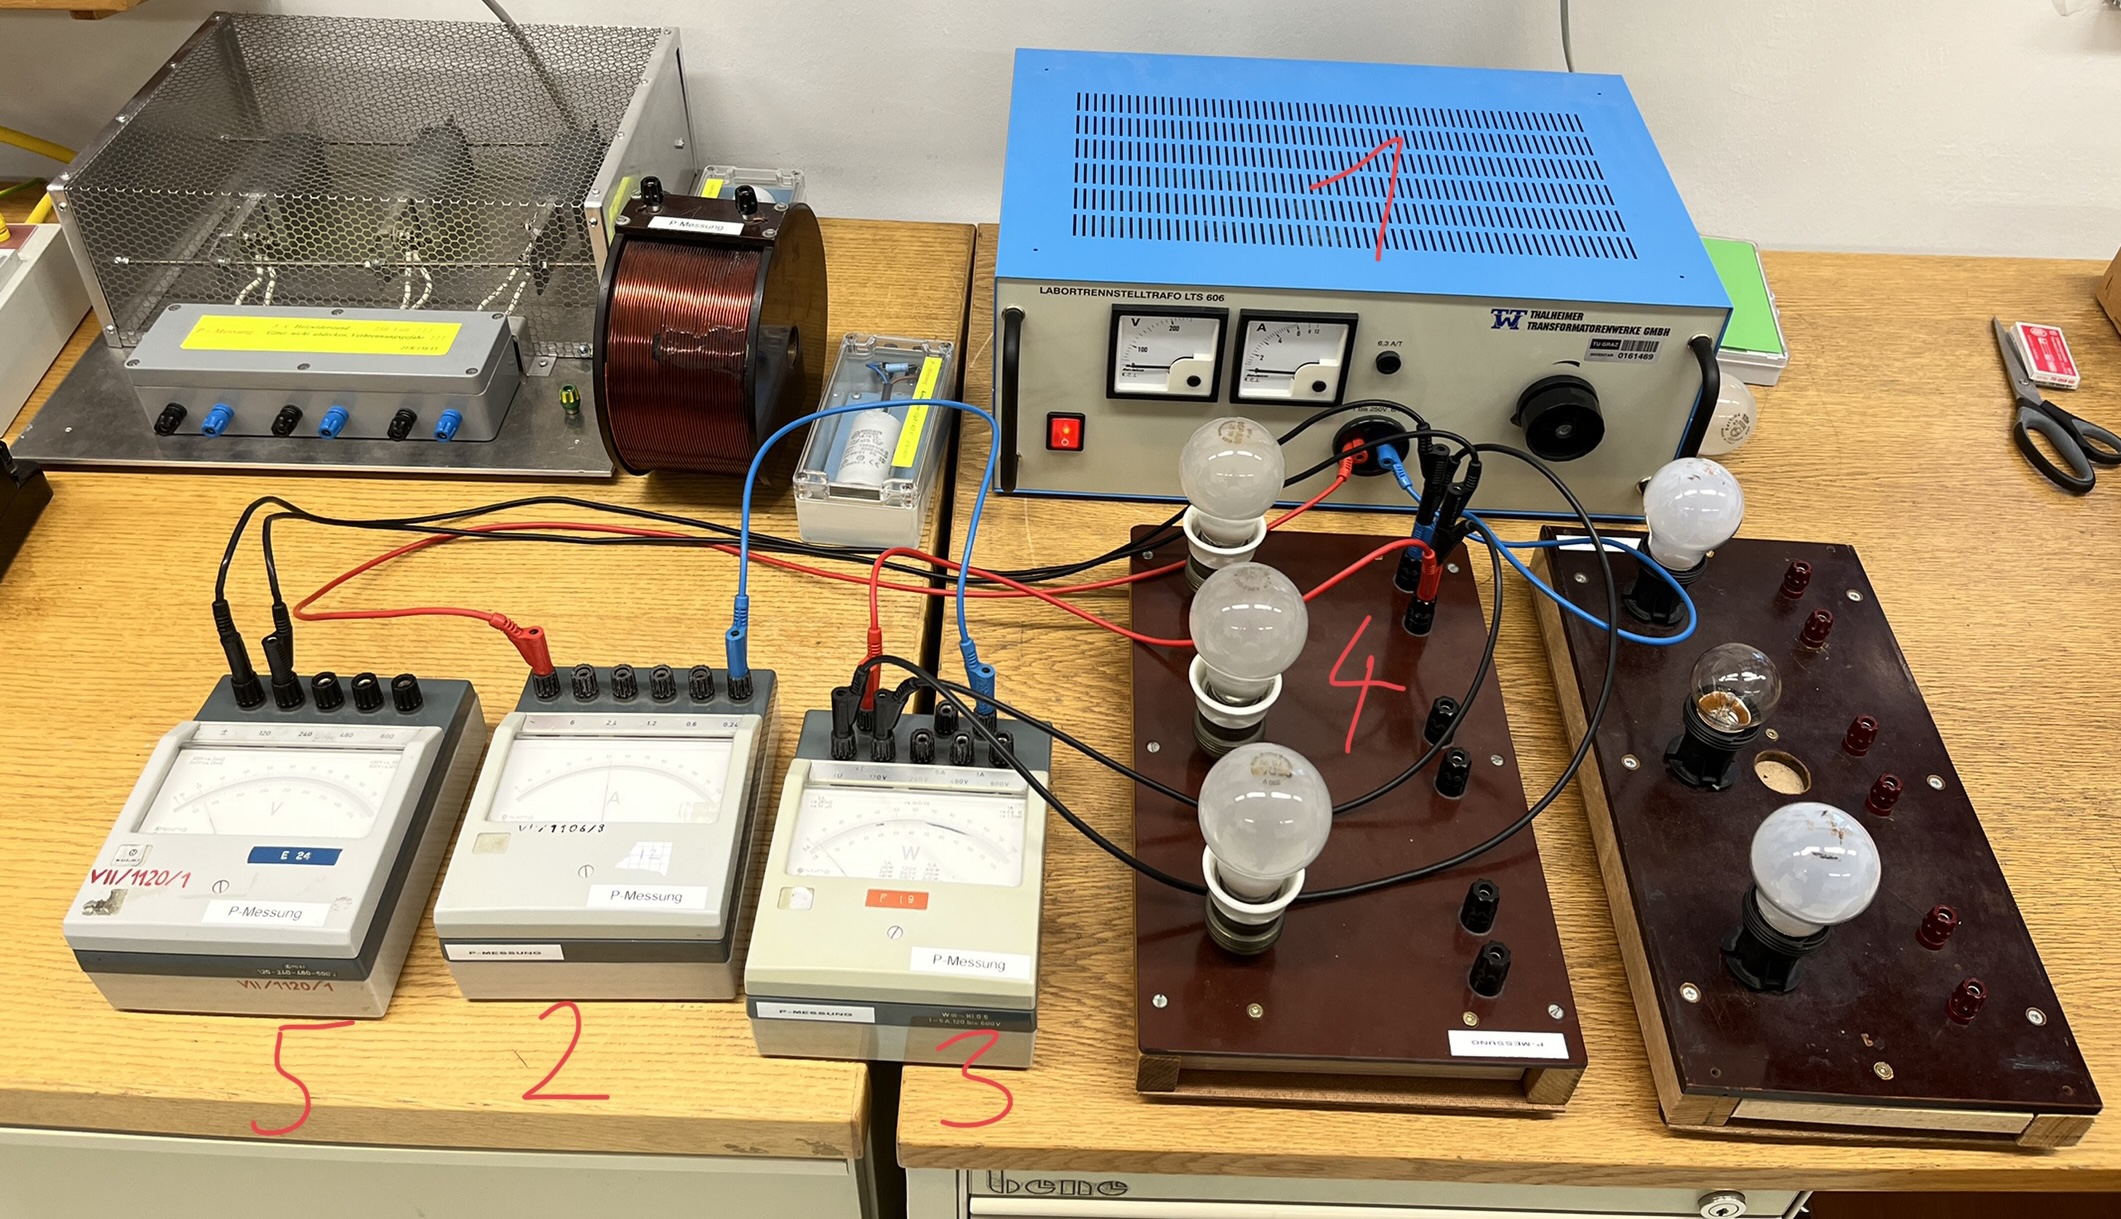
\includegraphics[width = 0.5\textwidth]{./figures/aufbau_ohm.png}
	\end{center}
	\caption[Realer Versuchsaufbau für die Messung einer ohmschen Last] {Realer
		Versuchsaufbau für die Messung einer ohmschen Last \\
		1 \(\dots\) Transformator                          \\
		2 \(\dots\) seriell geschaltetes Strommessgerät    \\
		3 \(\dots\) seriell geschaltetes Leistungsmessgerät mit parallelen Anschluss
		zum Verbraucher                                    \\
		4 \(\dots\) ohmscher Verbraucher (Glühlampe)       \\
		5 \(\dots\) parallel geschaltetes Spannungsmessgerät
	}\label{fig:aufbau_ohm}
\end{figure}

\subsection{Symmetrische Last in Dreieckschaltung}

Um die Wirkleistung von symmetrischen Verbrauchern in einer Dreiecksschaltung
zu Messen, wird die Aronschaltung nach folgendem Schaltplan aus
\autoref{fig:aufbau1} realisiert. Der tatsächliche Versuchsaufbau ist in
\autoref{fig:aufbau1_echt} ersichtlich.

\begin{figure}[H]
	\begin{center}
		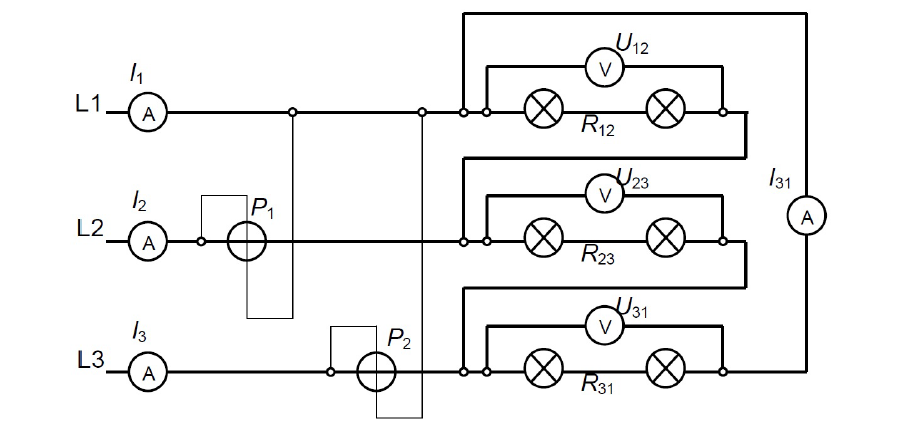
\includegraphics[width = 0.8\textwidth]{./figures/aufbau1.png}
	\end{center}
	\caption[Schaltplan für die Messung der Wirkleistung mit Aronschaltung für symmetrische
		Verbraucher in Dreiecksschaltung] {Schaltplan für die Messung der Wirkleistung
		mit Aronschaltung für symmetrische Verbraucher in
		Dreiecksschaltung~\cite[]{leistungsmessungvorbereitung}                          \\
		$I_i$ \(\dots\) entsprechende Ströme gemessen mit entsprechenden Amperemeter A   \\
		$U_i$ \(\dots\) entsprechende Spannungen gemessen mit entsprechenden Voltmeter V \\
		$R_i$ \(\dots\) entsprechender Widerstand durch die jeweiligen Verbraucher       \\
		$P_i$ \(\dots\) Powermeter in Aronschaltung
	}\label{fig:aufbau1}
\end{figure}

\begin{figure}[H]
	\begin{center}
		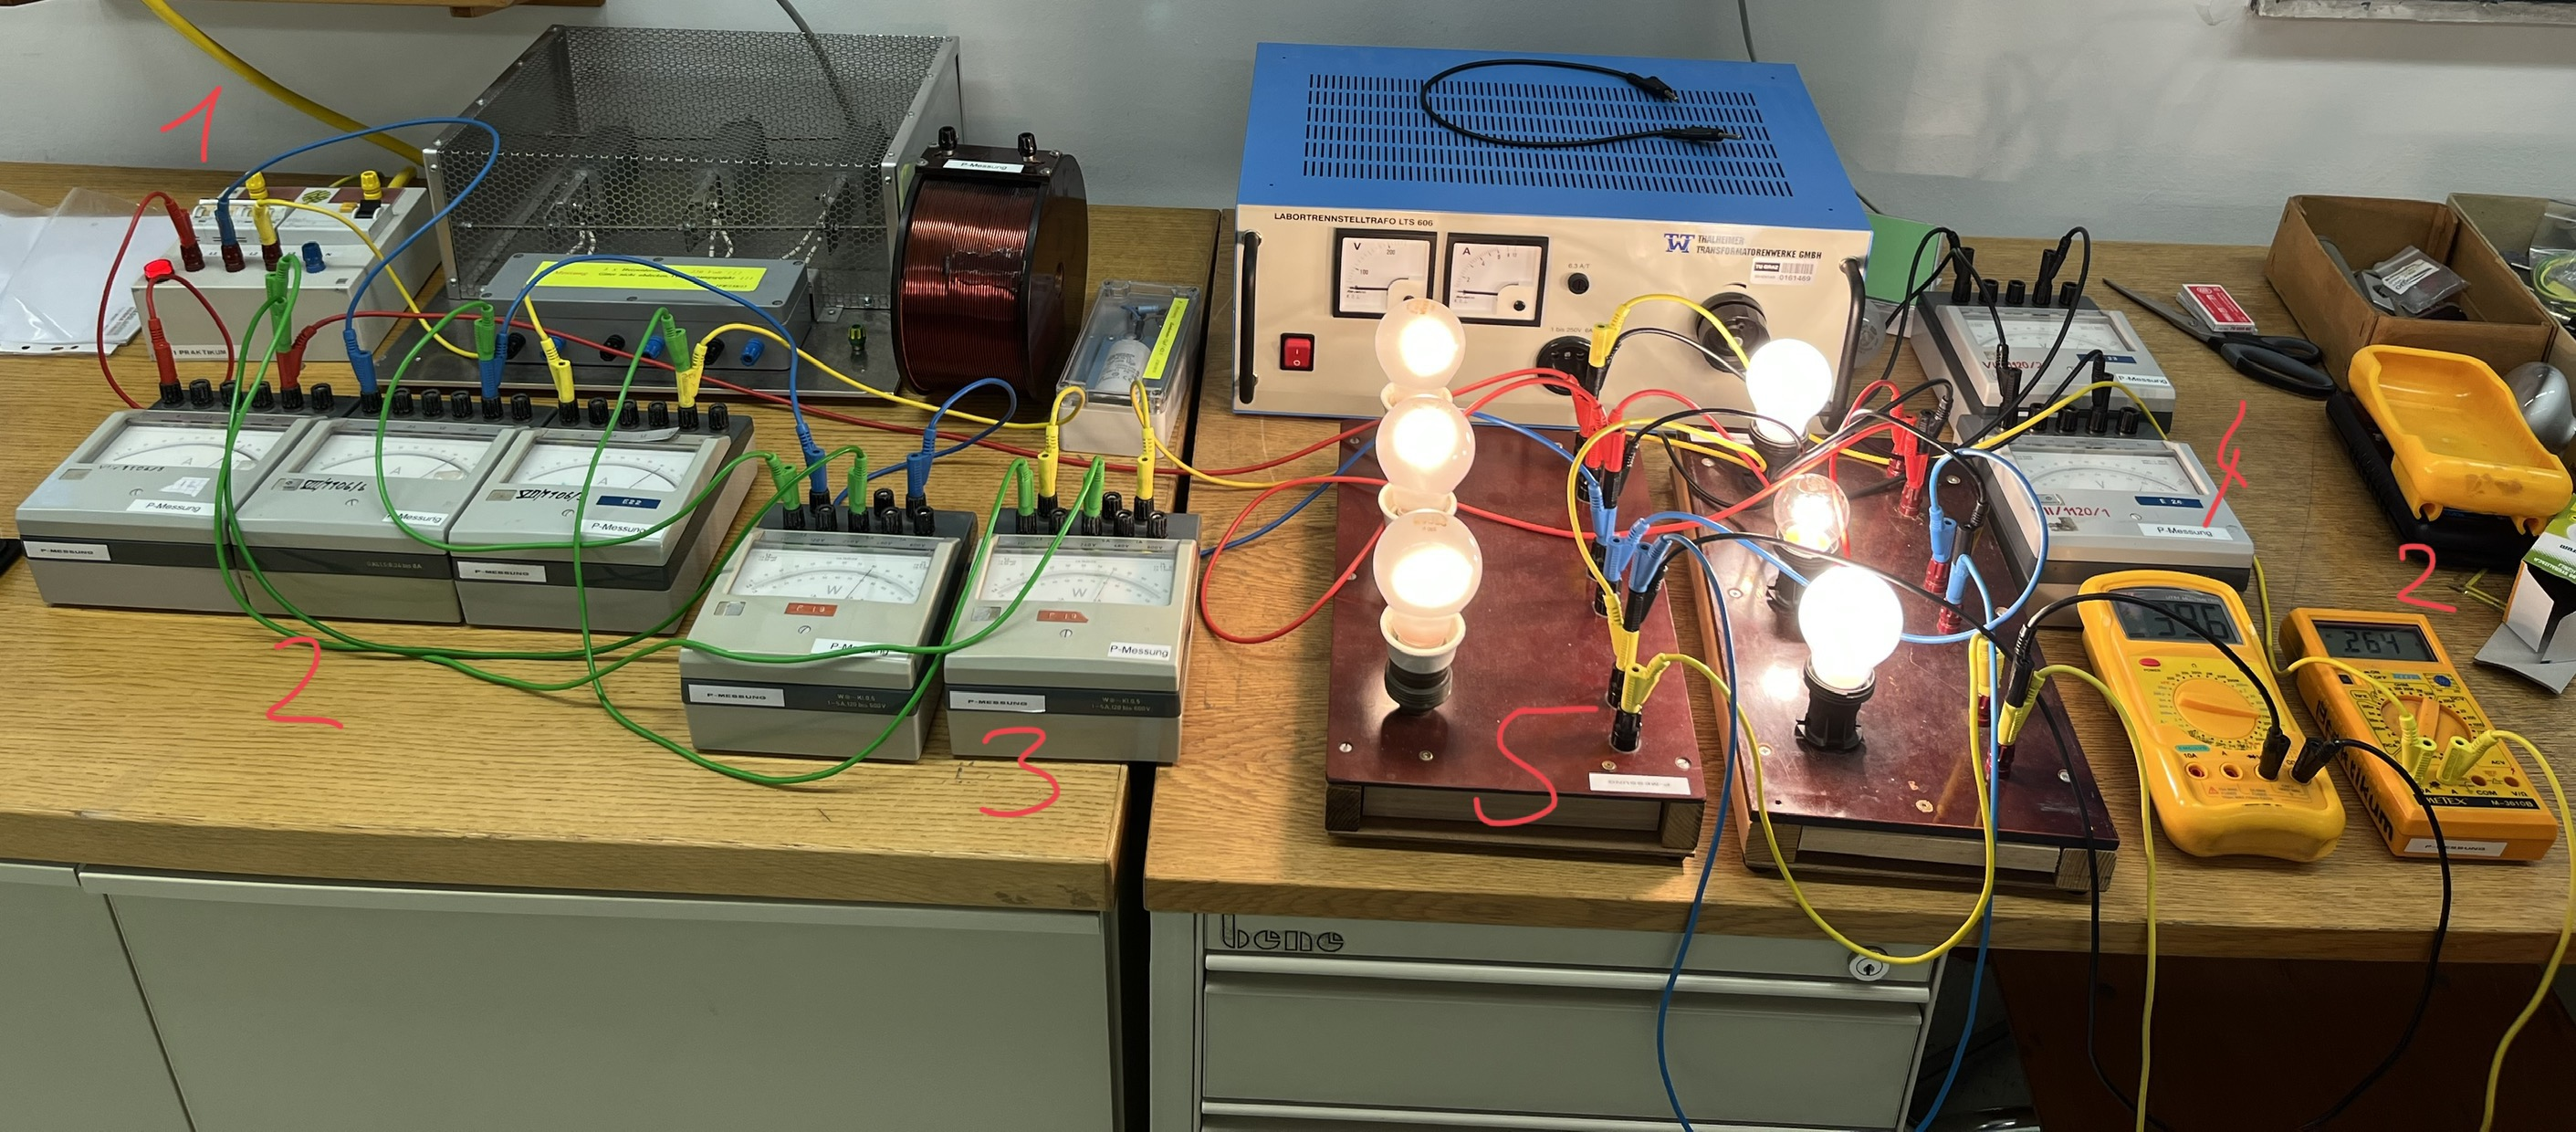
\includegraphics[width = \textwidth]{./figures/aufbau1_echt.png}
	\end{center}
	\caption[Realer Versuchsaufbau für die Messung der Wirkleistung mit Aronschaltung für
		symmetrische Verbraucher in Dreiecksschaltung] {Realer Versuchsaufbau für die
		Messung der Wirkleistung mit Aronschaltung für symmetrische Verbraucher in
		Dreiecksschaltung. (Bei den Kabeln wurde ein Farbschema eingehalten, um eine
		bessere Übersicht zu ermöglichen.)                                  \\
		1 \(\dots\) Versorgungsspannung ($L_1$ rot, $L_2$ blau, $L_3$ gelb) \\
		2 \(\dots\) seriell geschaltete Strommessgeräte                     \\
		3 \(\dots\) seriell geschaltete Leistungsmessgeräte mit parallelen Anschlüssen
		nach der Aronschaltung (grün)                                       \\
		4 \(\dots\) parallel geschaltete Spannungsmessgeräte über die entsprechenden
		Verbraucher (schwarz)                                               \\
		5 \(\dots\) symmetrisch verteilte ohmsche Verbraucher (Glühlampen)
	}
	\label{fig:aufbau1_echt}
\end{figure}

\subsection{Symmetrische Last in Sternschaltung}

Um die Wirkleistung von symmetrischen Verbrauchern in einer Sternschaltung zu
Messen, wird die Aronschaltung nach folgendem Schaltplan aus
\autoref{fig:aufbau2} realisiert. Der tatsächliche Versuchsaufbau ist in
\autoref{fig:aufbau2_echt} ersichtlich.

\begin{figure}[H]
	\begin{center}
		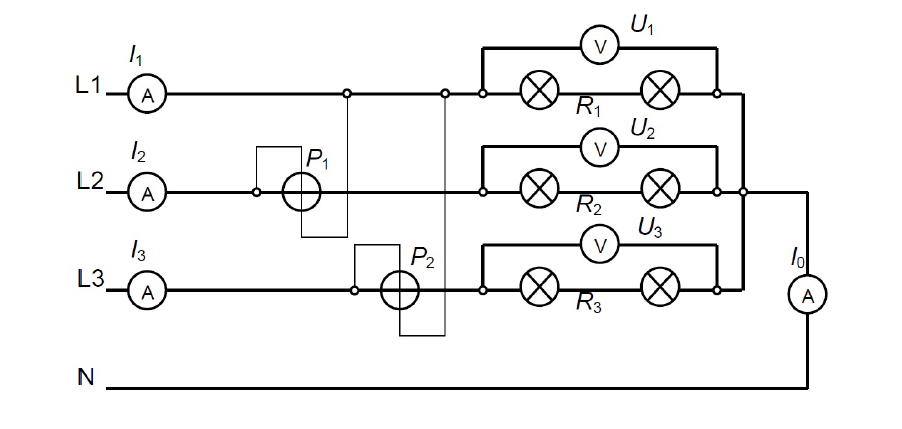
\includegraphics[width = 0.8\textwidth]{./figures/aufbau2.png}
	\end{center}
	\caption[Schaltplan für die Messung der Wirkleistung mit Aronschaltung für symmetrische
		Verbraucher in Sternschaltung] {Schaltplan für die Messung der Wirkleistung mit
		Aronschaltung für symmetrische Verbraucher in
		Sternschaltung~\cite[]{leistungsmessungvorbereitung}                             \\
		$I_i$ \(\dots\) entsprechende Ströme gemessen mit entsprechenden Amperemeter A   \\
		$U_i$ \(\dots\) entsprechende Spannungen gemessen mit entsprechenden Voltmeter V \\
		$R_i$ \(\dots\) entsprechender Widerstand durch die jeweiligen Verbraucher       \\
		$P_i$ \(\dots\) Powermeter in Aronschaltung
	}
	\label{fig:aufbau2}
\end{figure}

\begin{figure}[H]
	\begin{center}
		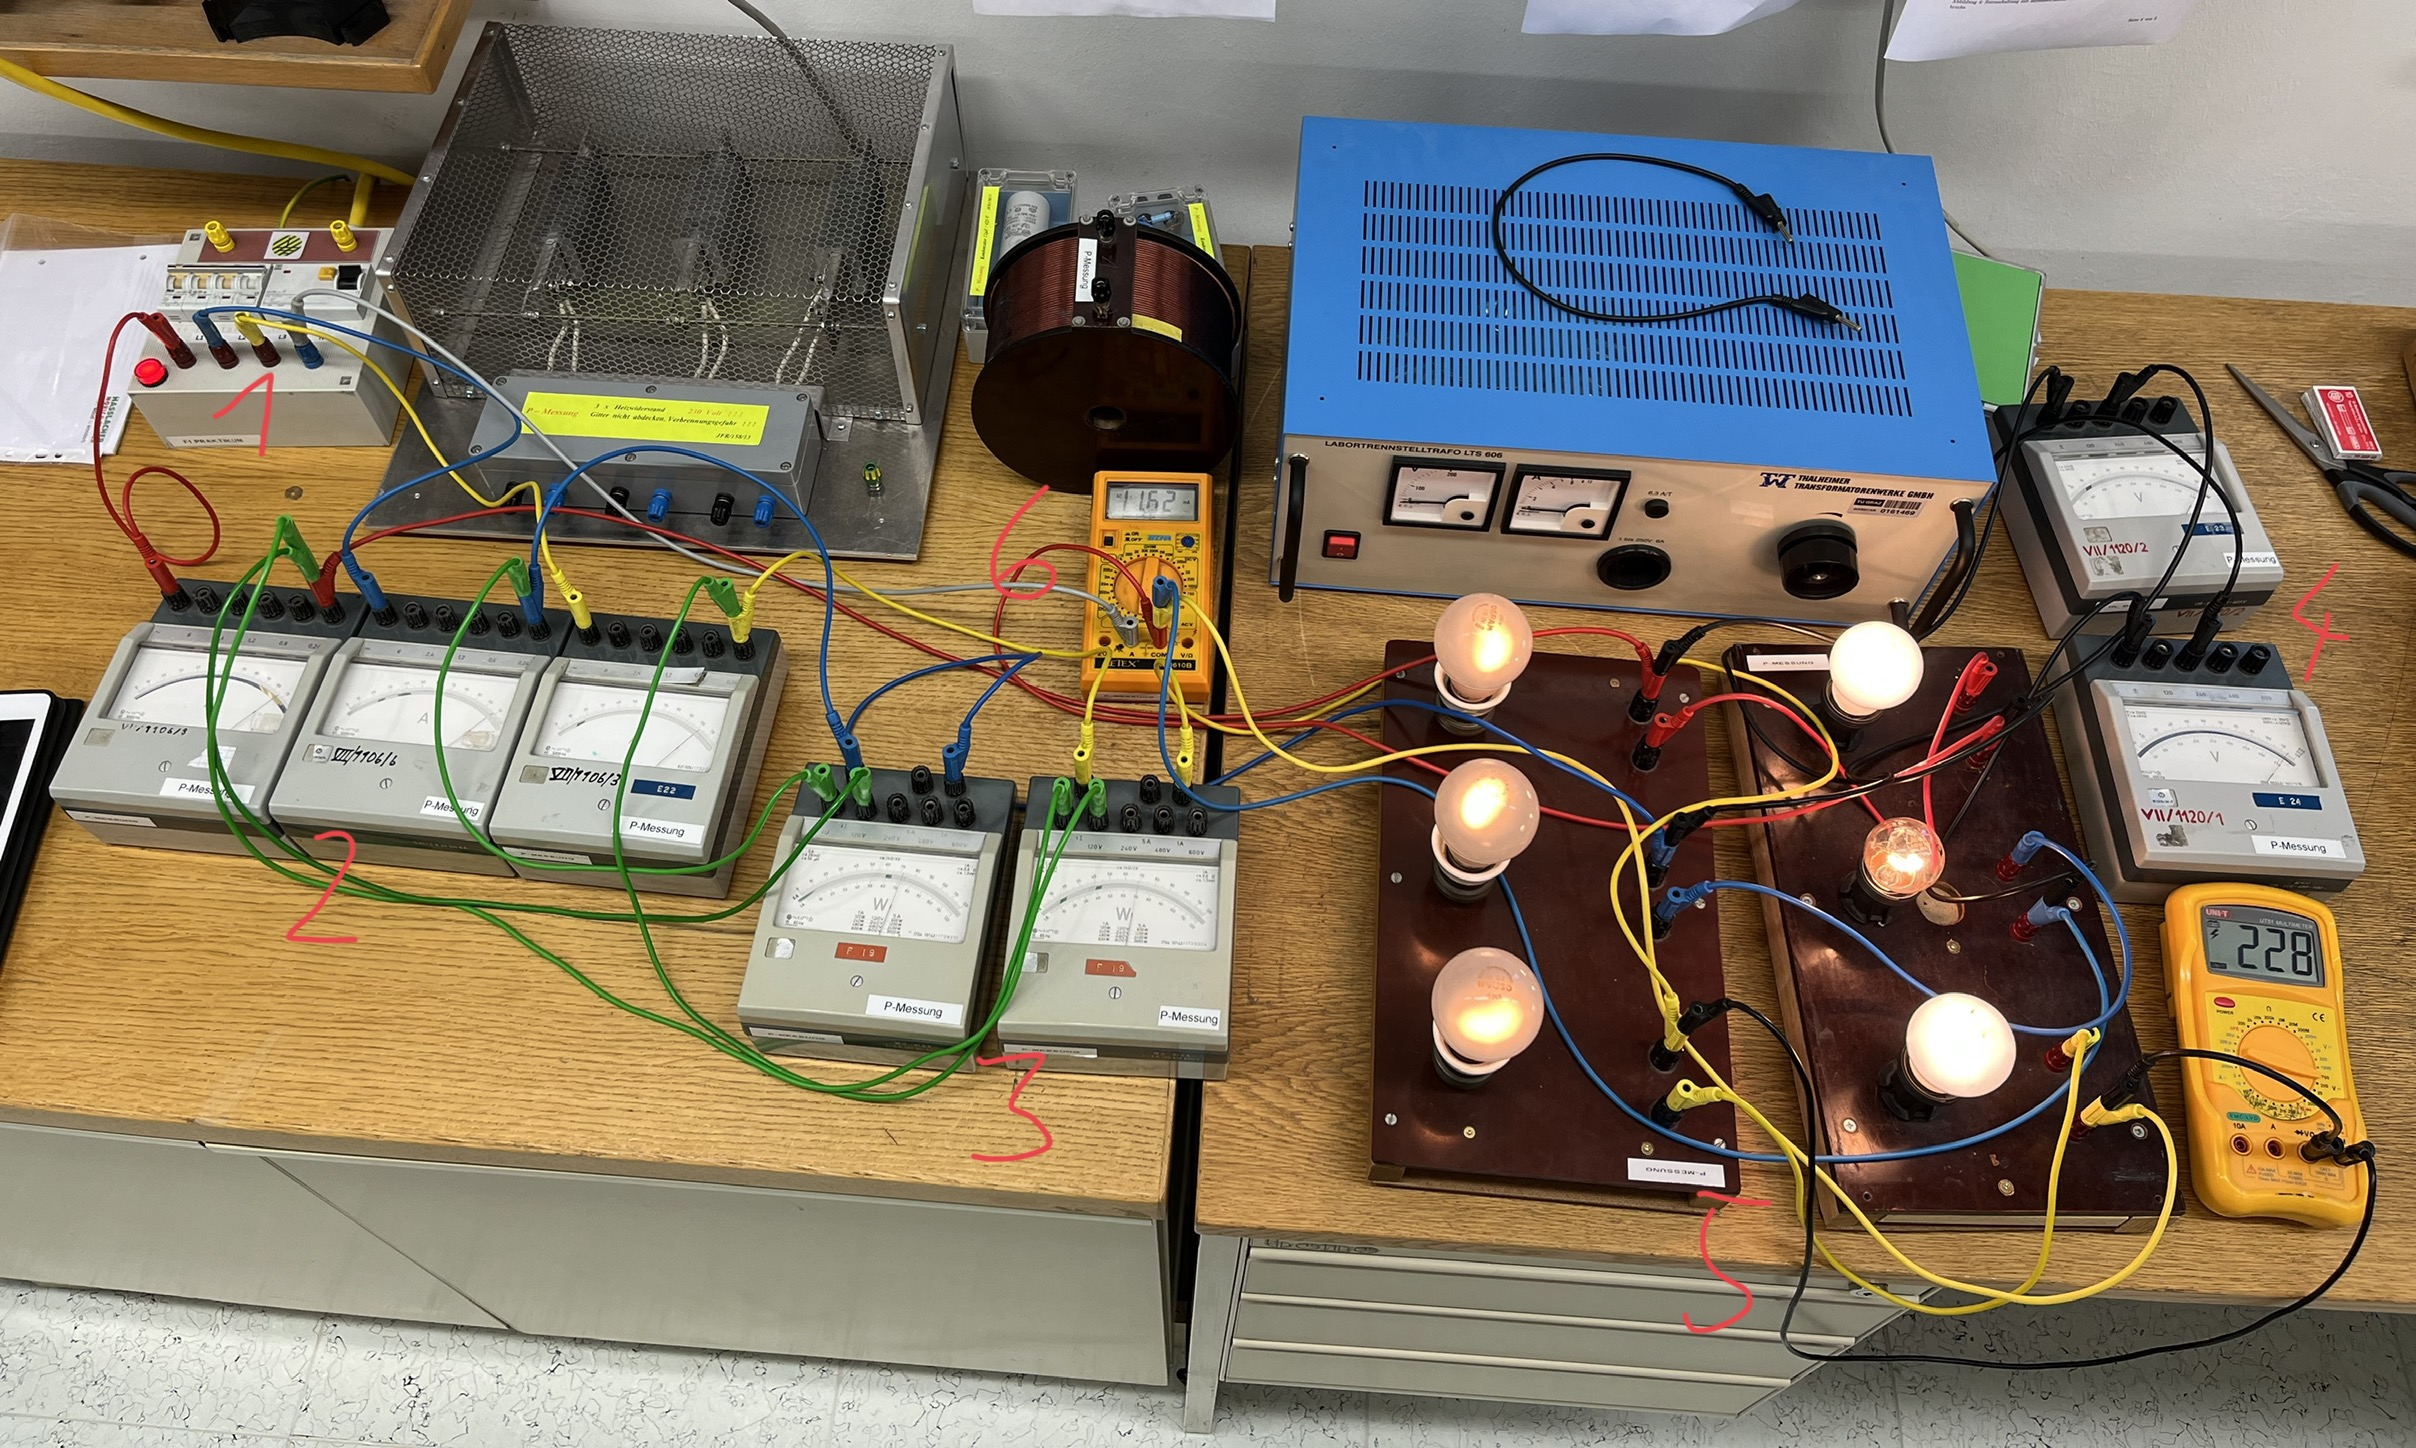
\includegraphics[width = \textwidth]{./figures/aufbau2_echt.png}
	\end{center}
	\caption[Realer Versuchsaufbau für die Messung der Wirkleistung mit Aronschaltung für
		symmetrische Verbraucher in Sternschaltung] {Realer Versuchsaufbau für die
		Messung der Wirkleistung mit Aronschaltung für symmetrische Verbraucher in
		Sternschaltung. (Bei den Kabeln wurde ein Farbschema eingehalten, um eine
		bessere Übersicht zu ermöglichen.)                                  \\
		1 \(\dots\) Versorgungsspannung ($L_1$ rot, $L_2$ blau, $L_3$ gelb) \\
		2 \(\dots\) seriell geschaltete Strommessgeräte                     \\
		3 \(\dots\) seriell geschaltete Leistungsmessgeräte mit parallelen Anschlüssen
		nach der Aronschaltung (grün)                                       \\
		4 \(\dots\) parallel geschaltete Spannungsmessgeräte über die entsprechenden
		Verbraucher (schwarz)                                               \\
		5 \(\dots\) symmetrisch verteilte ohmsche Verbraucher (Glühlampen)  \\
		6 \(\dots\) Strommessgerät zwischen Sternpunkt und Neutralleiter (grau)
	}\label{fig:aufbau2_echt}
\end{figure}

\subsection{Asymmetrische Last in Sternschaltung}

Um eine asymmetrische Last zu erreichen, wird der Aufbau aus
\autoref{fig:aufbau2} herangezogen, mit dem Unterschied, dass die Glühlampen
nicht gleichmäßig auf die Leiter aufgeteilt werden. Die gewählte Konfiguration
ist in \autoref{fig:lampenasym} ersichtlich.

\begin{figure}[H]
	\begin{center}
		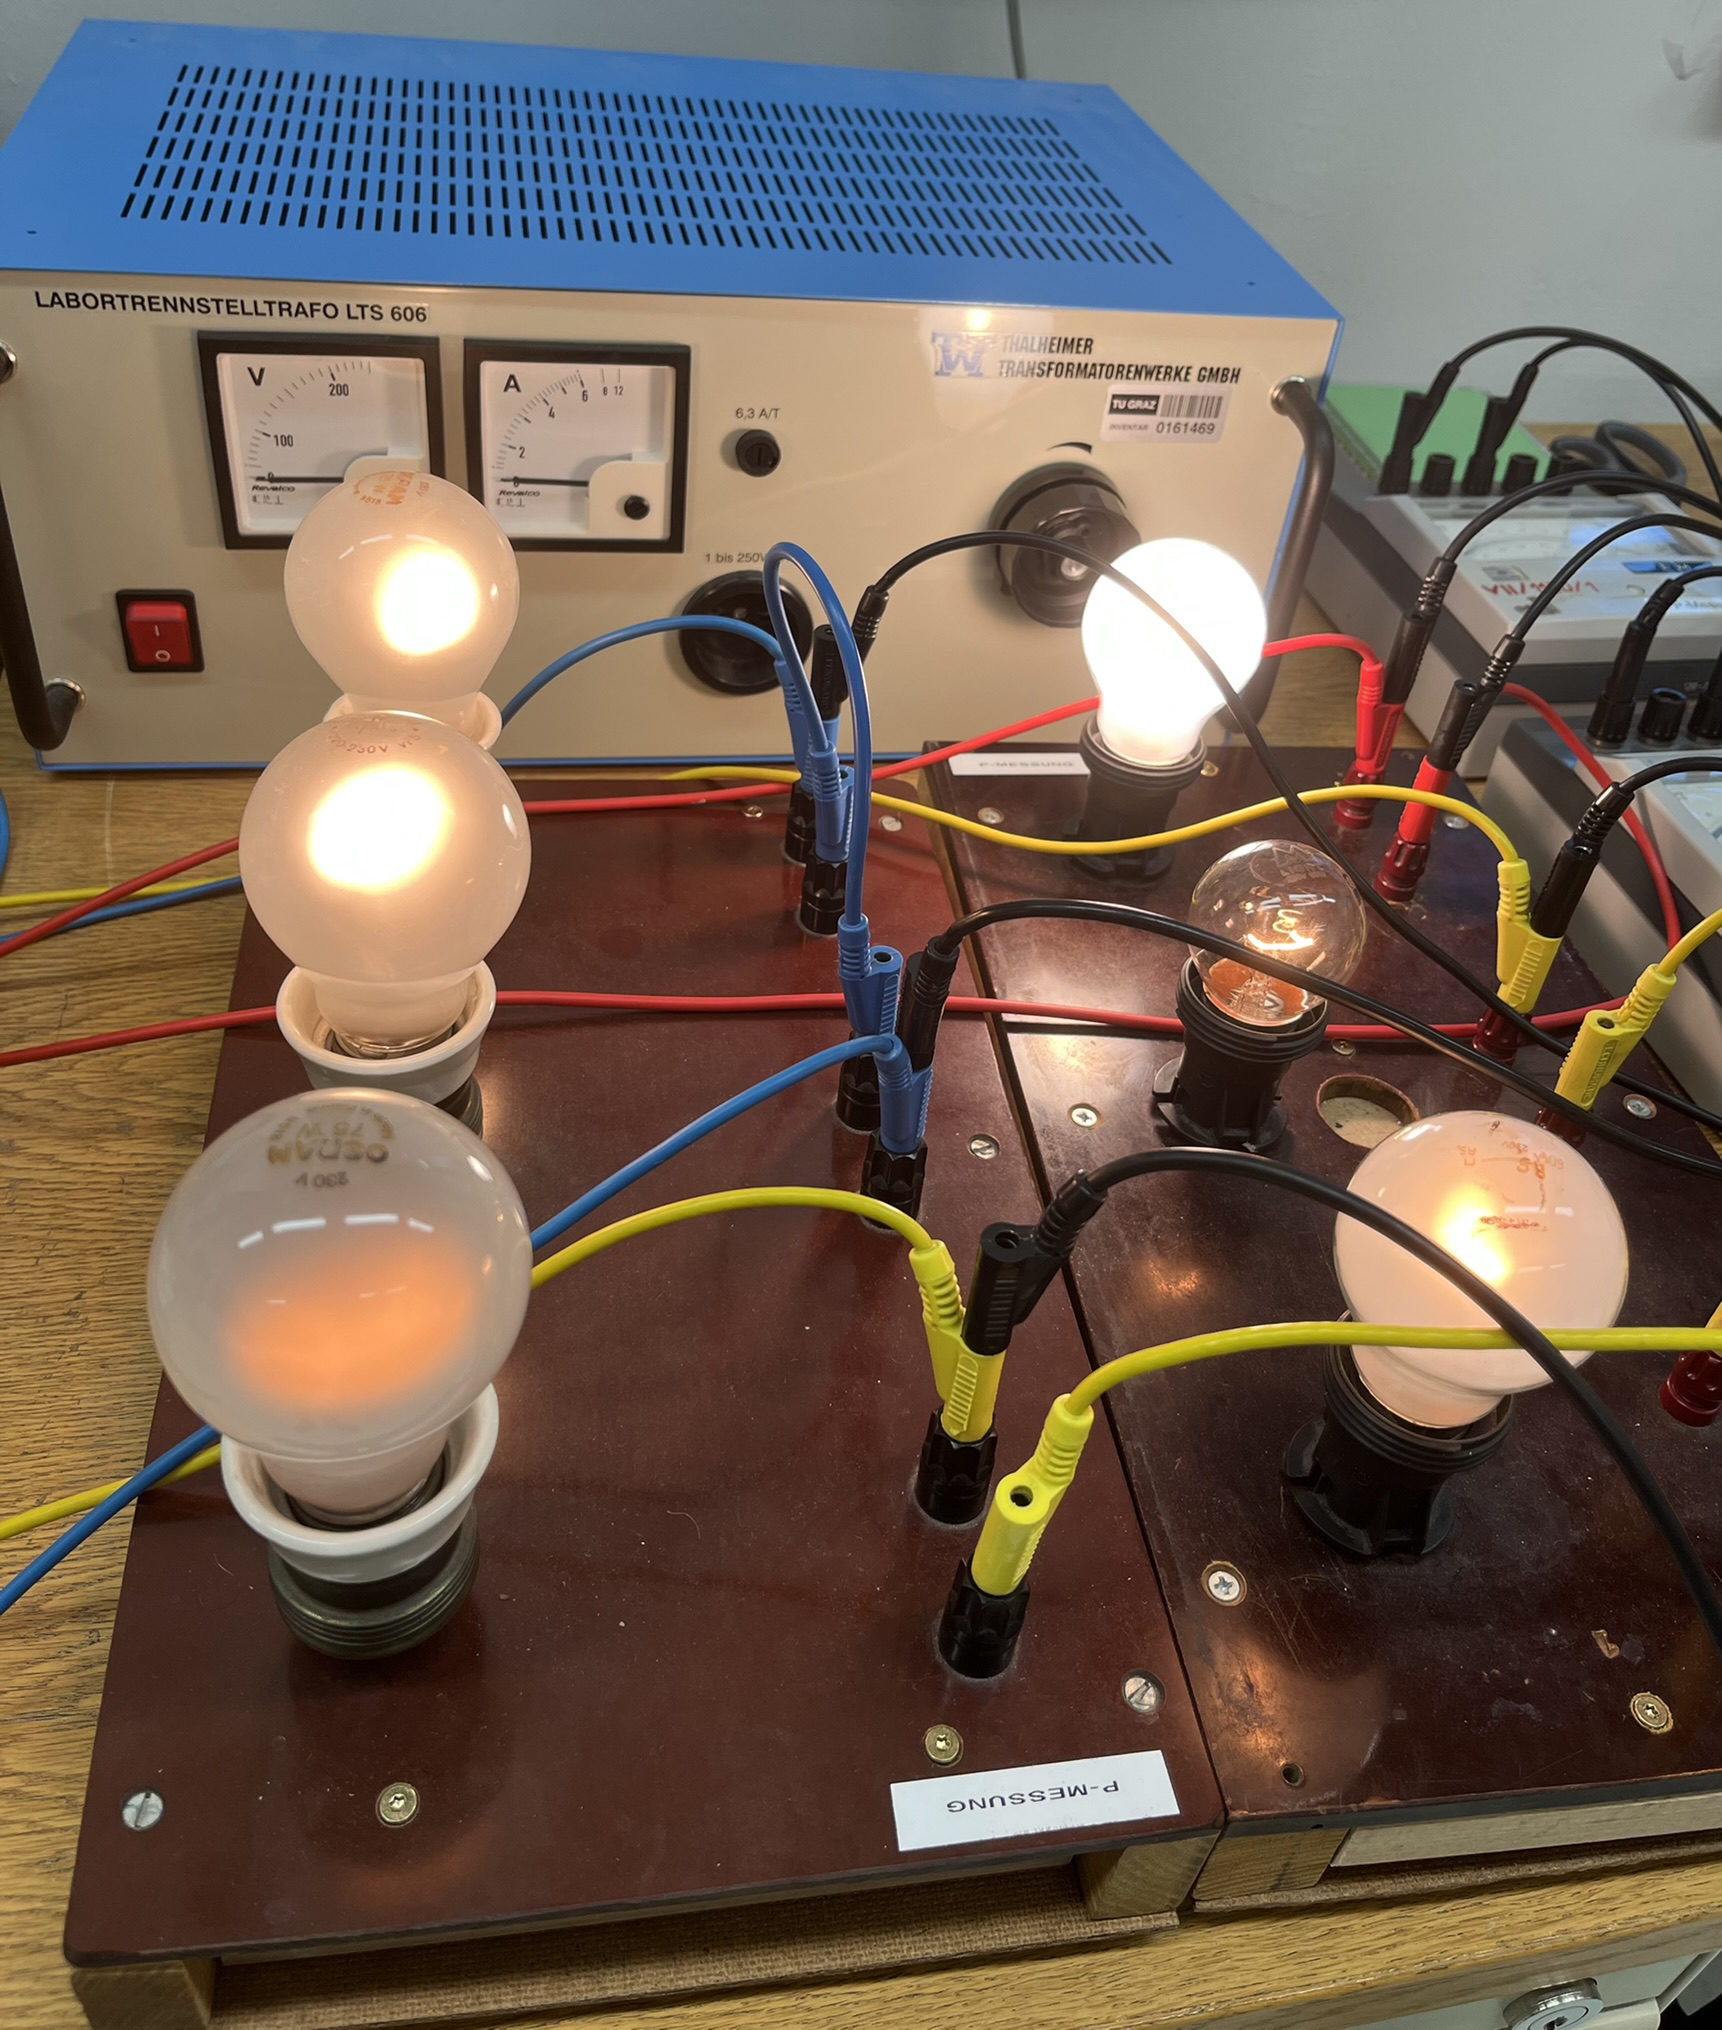
\includegraphics[width = 0.5\textwidth]{./figures/lampen.png}
	\end{center}
	\caption[Entsprechende Konfiguration für eine asymmetrische Verteilung der Last]
	{Entsprechende Konfiguration für eine asymmetrische Verteilung der Last mit
		folgenden Verteilungen auf den Strängen: \\
		$L_1$ \(\dots\) 1 x \SI[]{60}{\watt}     \\
		$L_2$ \(\dots\) 2 x \SI[]{75}{\watt}     \\
		$L_3$ \(\dots\) 1 x \SI[]{75}{\watt} und 2 x \SI[]{60}{\watt}
	}\label{fig:lampenasym}
\end{figure}

\subsection{Asymmetrische Last in Sternschaltung und simulierten Kabelbruch}

Um einen Kabelbruch zu simulieren, wird der Aufbau aus \autoref{fig:aufbau2}
herangezogen. Nun wird der Kontakt des Neutralleiters unterbrochen, indem das
graue Kabel, sichtbar in \autoref{fig:aufbau1_echt}, aus dem Strompfad des
Multimeters entfernt und in den Spannungsbereich gesteckt wird, um eine
Spannungsmessung zu ermöglichen.

\subsection{Wirkleistungsmessung}

Um die Wirkleistung von allgemeinen Verbrauchern in Sternschaltung zu
bestimmen, wird die Schaltung nach folgendem Schaltplan aus
\autoref{fig:aufbau3} aufgebaut. Der tatsächliche Versuchsaufbau ist in
\autoref{fig:aufbau3_echt} ersichtlich.

\begin{figure}[H]
	\begin{center}
		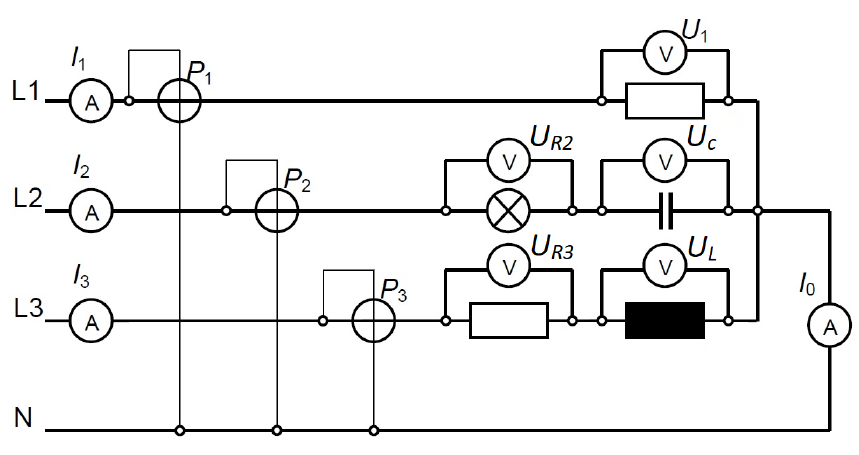
\includegraphics[width = 0.8\textwidth]{./figures/aufbau3.png}
	\end{center}
	\caption[Schaltplan für die Messung der Wirkleistung für allgemeine Verbraucher in
		Sternschaltung] {Schaltplan für die Messung der Wirkleistung für allgemeine
		Verbraucher in Sternschaltung~\cite[]{leistungsmessungvorbereitung}              \\
		$I_i$ \(\dots\) entsprechende Ströme gemessen mit entsprechenden Amperemeter A   \\
		$U_i$ \(\dots\) entsprechende Spannungen gemessen mit entsprechenden Voltmeter V \\
		$R_i$ \(\dots\) entsprechender Widerstand durch die jeweiligen Verbraucher       \\
		$P_i$ \(\dots\) Powermeter
	}
	\label{fig:aufbau3}
\end{figure}

\begin{figure}[H]
	\begin{center}
		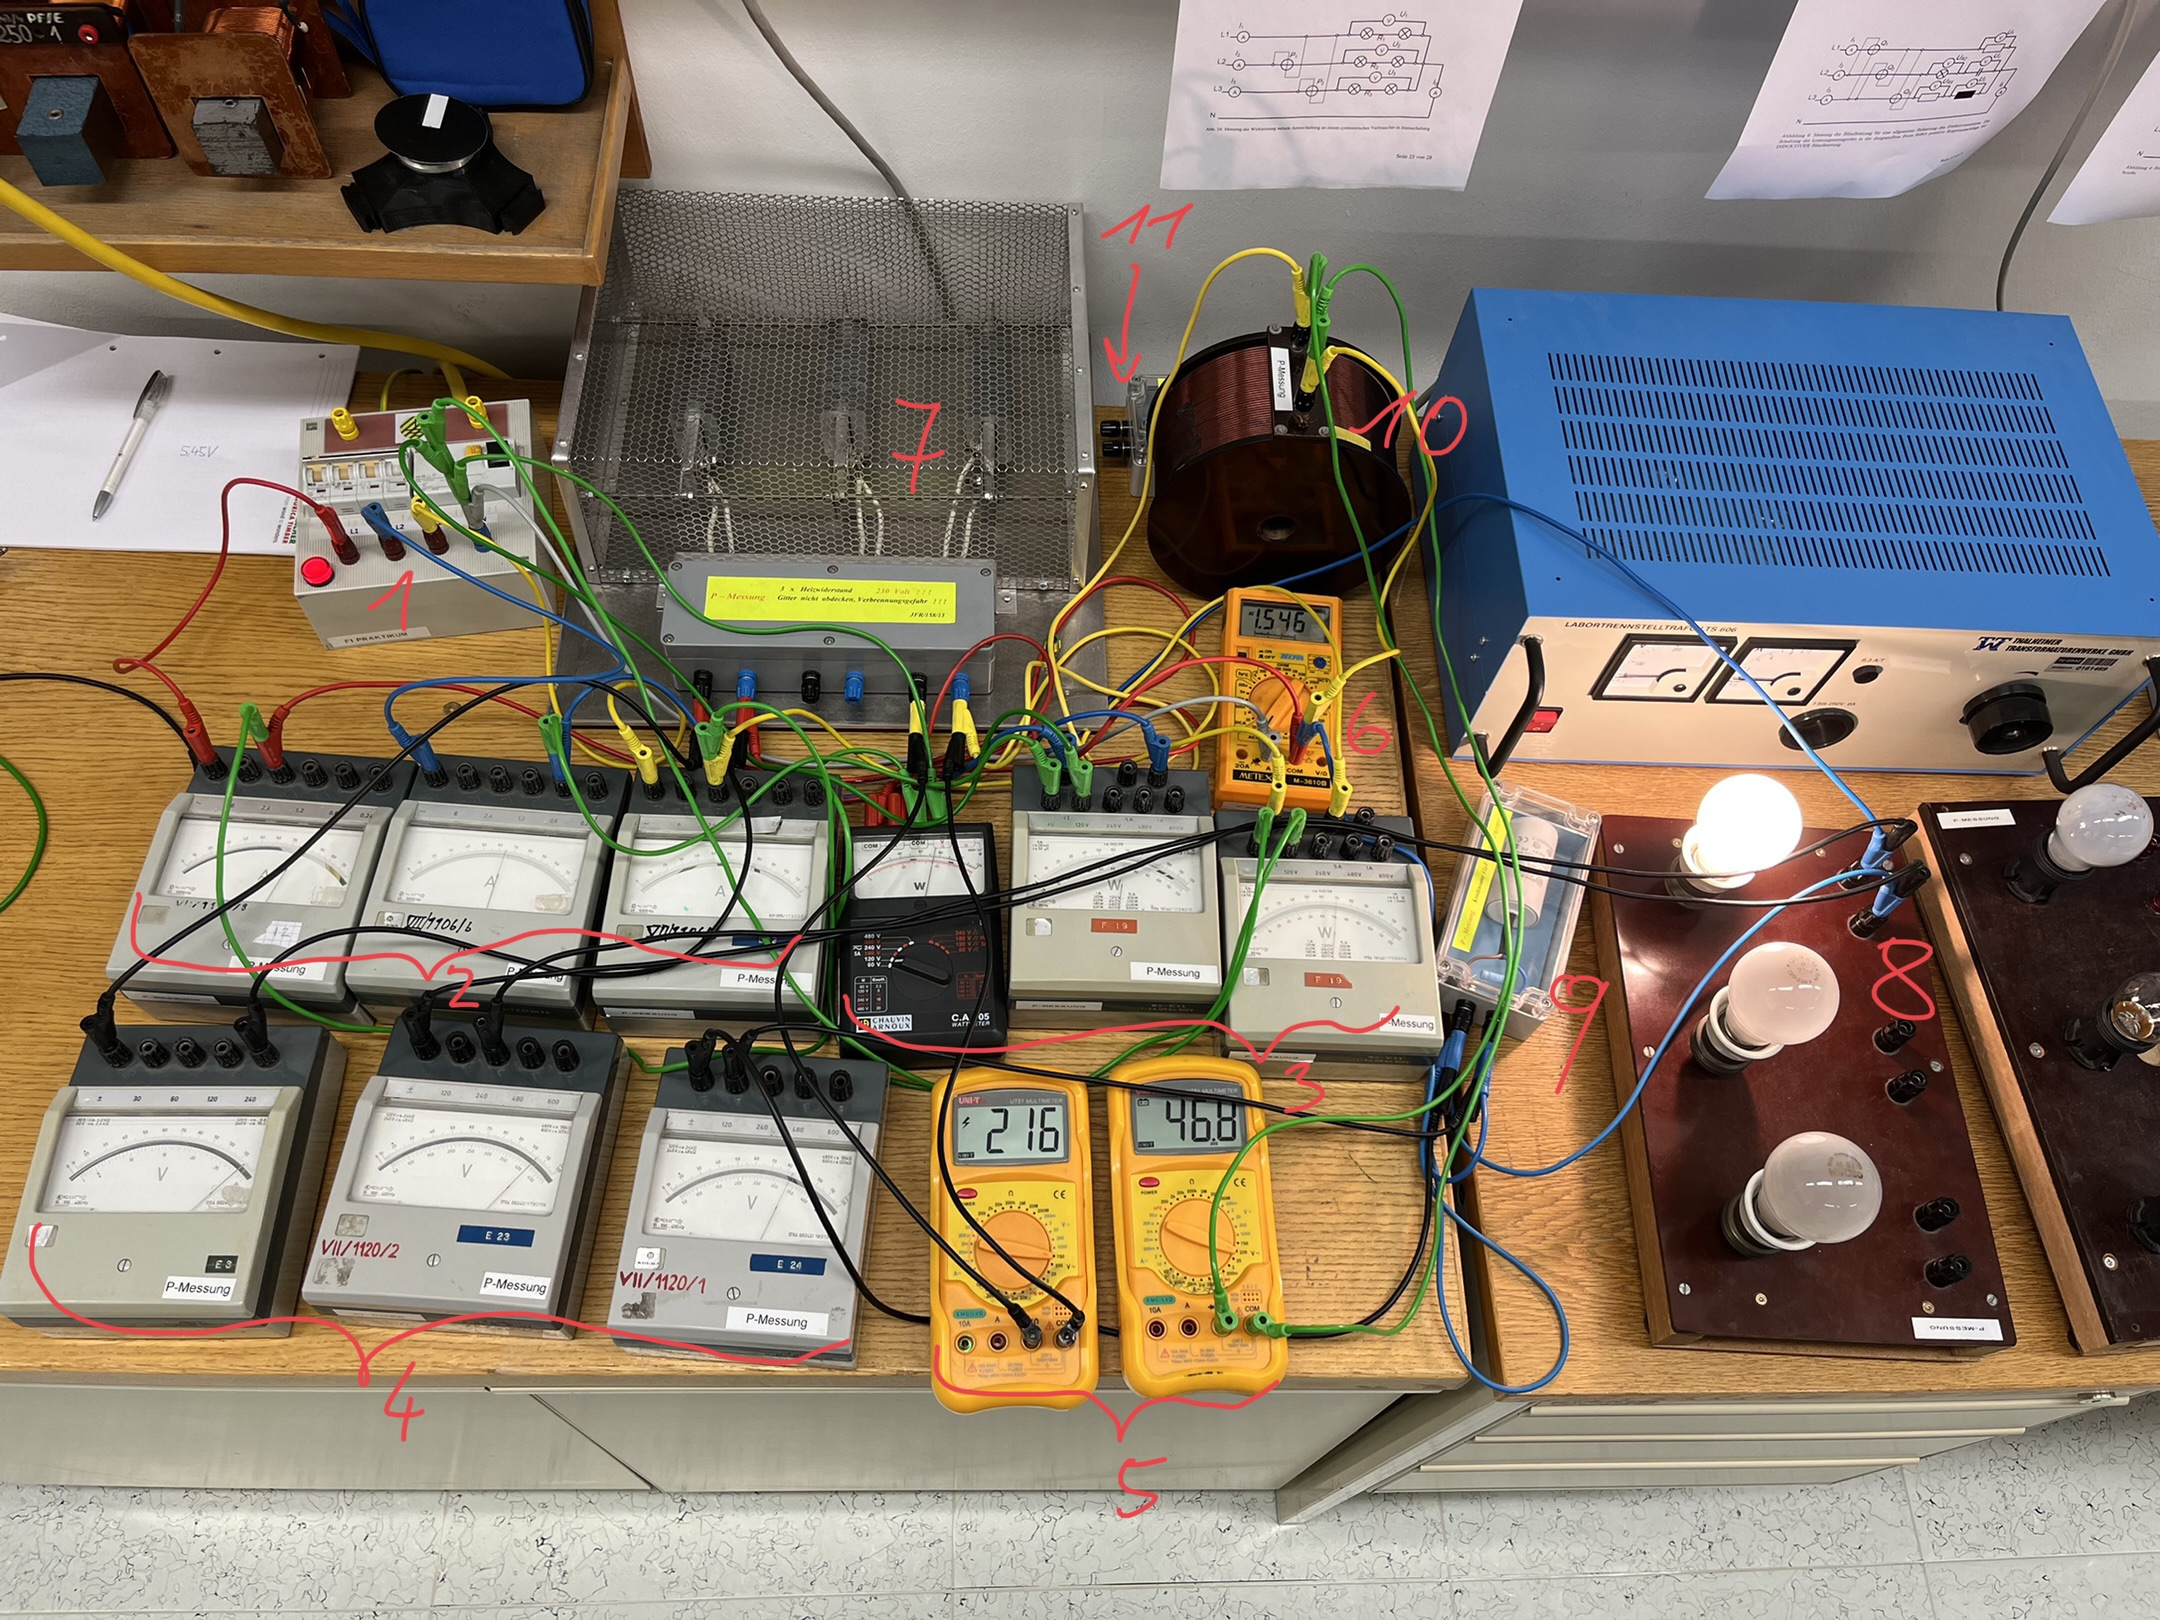
\includegraphics[width = \textwidth]{./figures/aufbau3_echt.png}
	\end{center}
	\caption[Realer Versuchsaufbau für die Messung der Wirkleistung für allgemeine
		Verbraucher in Sternschaltung] {Realer Versuchsaufbau für die Messung der
		Wirkleistung für allgemeine Verbraucher in Sternschaltung. (Bei den Kabeln
		wurde ein Farbschema eingehalten, um eine bessere Übersicht zu ermöglichen.) \\
		1 \(\dots\) Versorgungsspannung ($L_1$ rot, $L_2$ blau, $L_3$ gelb)          \\
		2 \(\dots\) seriell geschaltete Strommessgeräte                              \\
		3 \(\dots\) seriell geschaltete Leistungsmessgeräte mit parallelen Anschlüssen
		zum Neutralleiter (grün)                                                     \\
		4 \(\dots\) parallel geschaltete analoge Spannungsmessgeräte über die
		entsprechenden Verbraucher (schwarz)                                         \\
		5 \(\dots\) parallel geschaltete digitale Spannungsmessgeräte über die
		entsprechenden Verbraucher (schwarz/grün)                                    \\
		6 \(\dots\) Strommessgerät zwischen Sternpunkt und Neutralleiter (grau)      \\
		7 \(\dots\) Heizwiderstände                                                  \\
		8 \(\dots\) ohmscher Verbraucher                                             \\
		9 \(\dots\) Kapazität (Kondensator)                                          \\
		10 \(\dots\) Induktivität (Spule)                                            \\
		11 \(\dots\) 2. Kapazität für Bonusaufgabe

	}\label{fig:aufbau3_echt}
\end{figure}

Für die Bonusaufgabe werden folgende Änderungen vorgenommen:

\begin{itemize}
	\item $L_1$ bleibt unverändert (Heizwiderstand)
	\item $L_2$ Schaltung von einem Heizwiderstand und einem Kondensator mit parallel geschalteter Induktivität
	\item $L_3$ Schaltung von einem Heizwiderstand und einem Kondensator
\end{itemize}

\subsection{Blindleistungsmessung}

Um die Blindleistung eines allgemeinen Verbrauchers sichtbar zu machen, wird
nun die Schaltung nach folgendem Schaltplan aus \autoref{fig:aufbau4}
aufgebaut, indem die grünen Kabel der Powermeter aus \autoref{fig:aufbau3_echt}
entsprechend modifiziert werden.

\begin{figure}[H]
	\begin{center}
		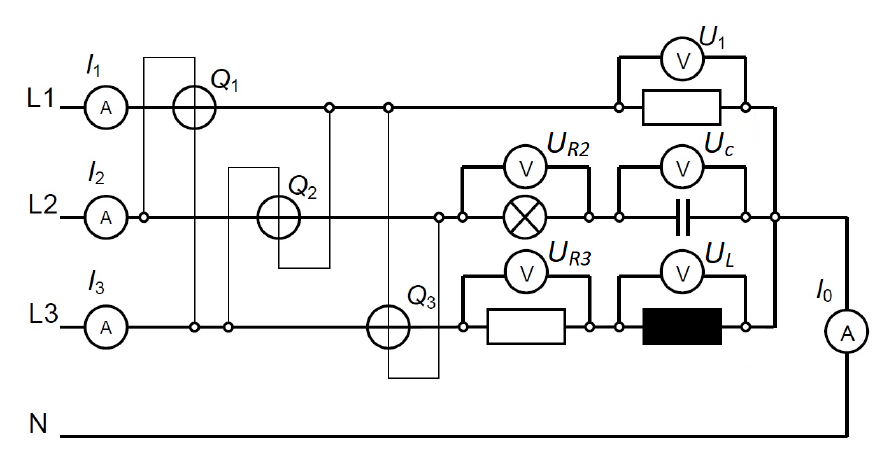
\includegraphics[width = 0.8\textwidth]{./figures/aufbau4.png}
	\end{center}
	\caption[Schaltplan für die Messung der Blindleistung für allgemeine Verbraucher in
		Sternschaltung] {Schaltplan für die Messung der Blindleistung für allgemeine
		Verbraucher in Sternschaltung~\cite[]{leistungsmessungvorbereitung}              \\
		$I_i$ \(\dots\) entsprechende Ströme gemessen mit entsprechenden Amperemeter A   \\
		$U_i$ \(\dots\) entsprechende Spannungen gemessen mit entsprechenden Voltmeter V \\
		$R_i$ \(\dots\) entsprechender Widerstand durch die jeweiligen Verbraucher       \\
		$P_i$ \(\dots\) Powermeter
	}
	\label{fig:aufbau4}
\end{figure}

\subsection{Bau eines rudimentären Asynchron-Drehstrommotors}

Um den Bau eines rudimentären Asynchron-Drehstrommotors zu realisieren, werden
3 Spulen mit Eisenkern wie in \autoref{fig:motor} um eine drehbar gelagerte
Metallscheibe aufgestellt. Die Spulen werden mit vorgeschalteten
Heizwiderständen an die Versorgungsspannung geschlossen.

\begin{figure}[H]
	\begin{center}
		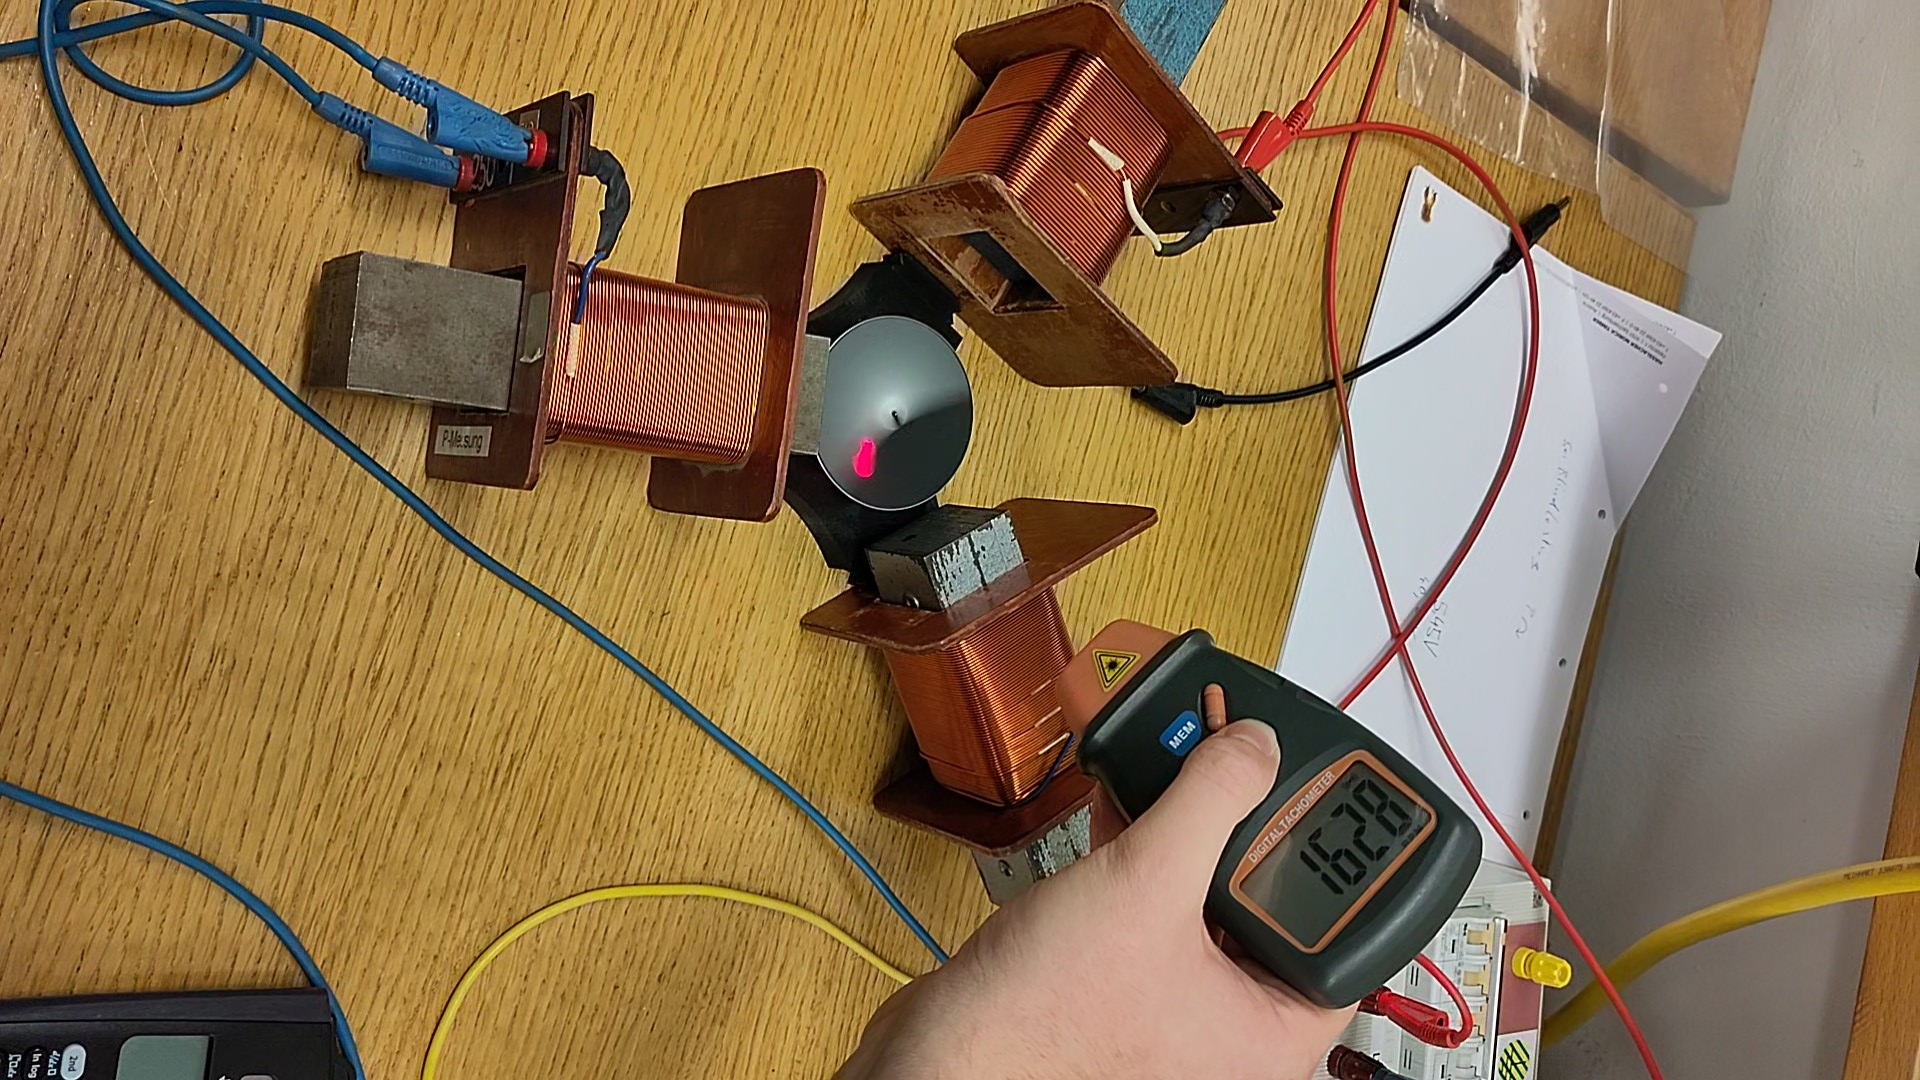
\includegraphics[width = 0.95\textwidth]{figures/motor.jpg}
	\end{center}
	\caption[Drehzahlmessung des rudimentären Asynchron-Drehstrommotors]{ Drehzahlmessung
		des rudimentären Asynchron-Drehstrommotors.
	}\label{fig:motor}
\end{figure}

\section{Geräteliste}\label{sec:geraeteliste}

Für den Versuch werden die in \autoref{tab:gerate} aufgelisteten Geräte
verwendet.

\begin{table}[H]
	\caption{Verwendete Geräte
	}
	\begin{tblr}{lllll}
		\textbf{Gerätetyp}  & \textbf{Hersteller} & \textbf{Typ}          & \textbf{Inventar-Nr} & \textbf{Anmerkung} \\
		Transformator       & Thalheimer          & LTS 606               & 0161469              &                    \\
		{Box  mit                                                                                                     \\ Versorgungsspannung} & & & F1 & \\
		Strommessgerät      & Norma               & analog                & {VII/1106/9                               \\ VII/1106/6 \\ VII/1106/3} & 3 x \\
		Spannungsmessgerät  & Norma               & analog                & {VII/1120/2                               \\ VII/1120/1 E3} & 3 x \\
		Leistungsmessgerät  & Norma               & analog                & F18 F19              & 2 x                \\
		Leistungsmessgerät  & {Chauvin                                                                                \\ Arnoux} & analog & C.A.505 & \\
		Multimeter          & UNI-T               & UT51                  &                      & 2 x                \\
		Multimeter          & METEX               & M-3610B               &                      &                    \\
		Glühbirnen          &                     & {3x \SI{60}{\watt}                                                \\ 3x \SI{75}{\watt}} & & \\
		Kondensator         &                     & \SI{12}{\micro\farad} & G5 V                 & 2 x                \\
		Spule               &                     &                       & P                    &                    \\
		Heizwiderstand      &                     & 3x \SI{230}{\volt}    & JFR/158/13           & 3 x                \\
		Bananenstecker      &                     &                       &                      &                    \\
		Spule mit Eisenkern &                     &                       &                      & 3 x                \\
		{Metallscheibe auf                                                                                            \\ Sockel} & Hancaner & DT2234C & & \\
	\end{tblr}\label{tab:gerate}
\end{table}

\section{Versuchsdurchführung und Messergebnisse}\label{sec:versuchsdurchfuehrung_messergebnisse}

\subsection{ohmsche Last in Wechselstromkreis}

Um die Leistung der ohmschen Last im Wechselstromkreis zu messen, wird der
Verbraucher, der in diesem Fall einer \SI[]{75}{\watt} Glühbirne entspricht,
wie in \autoref{fig:aufbau_ohm} ersichtlich, in den Stromkreis geschlossen.
Dabei ist besonders darauf zu achten, dass die Geräte richtig in den Stromkreis
geschlossen sind. Bei einem negativen Zeigerausschlag müssen also die Kabel
vertauscht werden. Auch sollt bei den Geräten der richtige Messbereich
ausgewählt werden, um sicherzustellen, dass die Geräte nicht überlastet werden,
aber dennoch ein genaues Ergebnis anzeigen.

Nun wird mithilfe des Schleifkontakts des Netzgeräts eine Ausgangsspannung von
\SI[]{20}{\volt} erzeugt und diese kontinuierlich erhöht, bis schließlich ein
Wert von \SI[]{240}{\volt} erreicht ist.
%todo 2x oben unsicherheit angeben
Die entsprechenden Werte der Messgeräte werden abgelesen und in folgender
\autoref{tab:werte_ohm} aufgelistet.

Bei dem vom Leistungsmessungsgerät abgelesenen Wert ist dabei besonders darauf
zu achten, ob das Gerät über die Verbindung für \SI{1}{\ampere} oder
\SI{5}{\ampere} verwendet wird.

\begin{table}[H]
	\caption[Gemessene Werte bei der Variation der ohmschen Last]{Gemessene Werte bei der
		Variation der ohmschen Last       \\
		$U \dots$ gemessene Spannung in V \\
		$I \dots$ gemessener Strom in A   \\
		$P \dots$ gemessene Leistung in W
	}\label{tab:werte_ohm}
	\centering
	\begin{tblr}{colspec={S[table-format=3.1(3)]S[table-format=1.3(1)]S[table-format=2.1(3)]}}
{{{$U$ / \si{\volt}}}} & {{{$I$ / \si{\ampere}}}} & {{{$P$ / \si{\watt}}}}\\
20.0(6) & 0.106(4) & 2.5(6)\\
40.0(6) & 0.136(4) & 6.0(6)\\
60.0(6) & 0.164(4) & 10.5(6)\\
80.0(6) & 0.191(4) & 16.0(6)\\
100.0(6) & 0.215(4) & 22.0(6)\\
120.0(6) & 0.238(4) & 30.0(6)\\
140.0(12) & 0.250(9) & 37.0(12)\\
160.0(12) & 0.270(9) & 46.0(12)\\
180.0(12) & 0.288(9) & 54.0(12)\\
200.0(12) & 0.305(9) & 64.0(12)\\
220.0(12) & 0.320(9) & 74.0(12)\\
240.0(12) & 0.335(9) & 84.0(12)\\
\end{tblr}

\end{table}

\subsection{Symmetrische Last in Dreieckschaltung}

Um die Leistung eines symmetrischen Verbrauchs bei einer Dreiecksschaltung zu
betrachten, wird ein Aufbau nach \autoref{fig:aufbau1} herangezogen. Dabei ist
darauf zu achten, dass die Glühlampen symmetrisch auf die Stränge verteilt
sind, sich also auf jeden jeweils eine mit \SI[]{75}{\watt} und eine mit
\SI[]{60}{\watt} befindet. Alle abgelesenen Messwerte der Messgeräte sind in
folgender \autoref{tab:werte_sym_dreieck} aufgelistet.

\begin{table}[H]
	\caption[Abgelesene Werte bei symmetrischer Belastung in Dreiecksschaltung] {Abgelesene
		Werte bei symmetrischer Belastung in Dreiecksschaltung                     \\
		$I_i \dots$ gemessener Strom am i-ten Strang in A                          \\
		$I_{31} \dots$ gemessener Strom zwischen Sternpunkt und Neutralleiter in A \\
		$U_{ij} \dots$ gemessene Spannung zwischen den Strängen i und j in V       \\
		$P_{i}^M \dots$ gemessene Wirkleistungen in W (für genaue Bezeichnung siehe \autoref{fig:aufbau1})
	}\label{tab:werte_sym_dreieck}
	\centering
	\begin{tblr}{colspec={S[table-format=1.3(2)]S[table-format=1.3(2)]S[table-format=1.3(2)]S[table-format=1.3(1)]}}
{{{$I_1$ / \si{\ampere}}}} & {{{$I_2$ / \si{\ampere}}}} & {{{$I_3$ / \si{\ampere}}}} & {{{$I_{31}$ / \si{\ampere}}}}\\
0.460(14) & 0.480(14) & 0.470(14) & 0.264(8)\\
\end{tblr}

	\begin{tblr}{colspec={S[table-format=3.0(1)]S[table-format=3.0(1)]S[table-format=3.0(1)]S[table-format=3.0(1)]S[table-format=3.0(1)]}}
{{{$U_{12}$ / \si{\volt}}}} & {{{$U_{23}$ / \si{\volt}}}} & {{{$U_{31}$ / \si{\volt}}}} & {{{$P_1^{M}$ / \si{\watt}}}} & {{{$P_2^{M}$ / \si{\watt}}}}\\
390(8) & 390(8) & 395(8) & 163(4) & 168(4)\\
\end{tblr}

\end{table}

\subsection{Symmetrische Last in Sternschaltung}

Nun wird die Schaltung insofern modifiziert, dass nun eine Sternschaltung
vorliegt, wie in \autoref{fig:aufbau2} sichtbar.

Der besseren Übersicht halber, sind alle abgelesenen Werte der Messgeräte für
die Sternschaltung in folgender \autoref{tab:wert_stern} aufgelistet.

\begin{table}[H]
	\caption[Abgelesene Werte bei Sternschaltung] {Abgelesene Werte bei Sternschaltung                                        \\
		1. Zeile \dots symmetrische Belastung                                      \\
		2. Zeile \dots asymmetrische Belastung                                     \\
		3. Zeile \dots asymmetrische Belastung mit simulierten Kabelbruch          \\
		$I_i \dots$ gemessener Strom am i-ten Strang in A                          \\
		$I_{31} \dots$ gemessener Strom zwischen Sternpunkt und Neutralleiter in A \\
		$U_{i} \dots$ gemessene Spannung am i-ten Strang in V                      \\
		$P_{i}^M \dots$ gemessene Wirkleistungen in W (für genaue Bezeichnung siehe \autoref{fig:aufbau2})
	}\label{tab:wert_stern}
	\centering
	\begin{tblr}{colspec={S[table-format=1.3(2)]S[table-format=1.3(2)]S[table-format=1.3(1)]S[table-format=1.4(1)]}}
{{{$I_1$ / \si{\ampere}}}} & {{{$I_2$ / \si{\ampere}}}} & {{{$I_3$ / \si{\ampere}}}} & {{{$I_{31}$ / \si{\ampere}}}}\\
0.218(6) & 0.220(6) & 0.226(6) & 0.0111(5)\\
0.270(14) & 0.255(14) & 0.172(6) & 0.092(5)\\
0.255(14) & 0.253(14) & 0.184(6) & {{{-}}}\\
\end{tblr}

	\begin{tblr}{colspec={S[table-format=3.0(1)]S[table-format=3.0(1)]S[table-format=3.0(1)]S[table-format=2.2(2)]S[table-format=2.1(3)]S[table-format=2.1(3)]}}
{{{$U_1$ / \si{\volt}}}} & {{{$U_2$ / \si{\volt}}}} & {{{$U_3$ / \si{\volt}}}} & {{{$P_1^{M}$ / \si{\watt}}}} & {{{$P_2^{M}$ / \si{\watt}}}} & {{{$P_3^{M}$ / \si{\watt}}}}\\
228(4) & 228(4) & 224(6) & 73.0(8) & 70.0(16) & {{{-}}}\\
230(4) & 230(4) & 224(6) & 19.5(2) & 82.0(16) & 55.0(16)\\
202(4) & 225(4) & 261(7) & 16.00(16) & 88.0(16) & 58.0(16)\\
\end{tblr}

\end{table}

\subsection{Asymmetrische Last in Sternschaltung}\label{sec:vers_asy_stern_ohne}

Nun werden die einzelnen Stränge verschieden stark beansprucht, indem die
Glühlampen asymmetrisch auf die Stränge verteilt werden. Dabei wird, wie
bereits in \autoref{sec:versuchsanordnung} angeführt, folgende Konfiguration
verwirklicht:

\begin{itemize}
	\item $L_1$ \(\dots\) 1 x \SI[]{60}{\watt}
	\item $L_2$ \(\dots\) 2 x \SI[]{75}{\watt}
	\item $L_3$ \(\dots\) 1 x \SI[]{75}{\watt} und 2 x \SI[]{60}{\watt}
\end{itemize}

Alle abgelesenen Werte der Messgeräte sind, wie bereits erwähnt, in folgender
\autoref{tab:wert_stern} in der 2. Zeile angefügt.

\subsection{Asymmetrische Last in Sternschaltung und simulierten Kabelbruch}\label{sec:vers_asy_stern_mit}

Um nun einen Kabelbruch zu simulieren, wird die Verbindung des Neutralleiters
unterbrochen. Zusätzlich wird nun auch der Spannungsabfall an jener Stelle
gemessen, indem das entsprechende Multimeter als Spannungsmessgerät
umfunktioniert wird. Die so abgelesenen Werte der Messgeräte sind in folgender
\autoref{tab:werte_stern} in der 3. Zeile aufgelistet.

\subsection{Wirkleistungsmessung}
Um die Wirkleistung eines realen Verbrauchers zu bestimmen, werden auch
Kapazitäten und Induktivitäten, wie in \autoref{fig:aufbau3} sichtbar, in die
Schaltung integriert.

Es sind, der besseren übersicht halber, wieder alle erhaltenen Werte für die
nächsten Aufgaben in \autoref{tab:werte_wirkleistung} aufgelistet. Die
gemessenen Werte der realen Verbraucher sind dabei in der 1. Zeile sichtbar.

%todo max schau bitte schnell ob richtig und verständlich
\begin{table}[H]
	\caption[Abgelesene Werte für die Bestimmung der Wirkleistung] {Abgelesene Werte für die
		Bestimmung der Wirkleistung                                                \\
		1. Zeile \dots Wirkleistung eines realen Verbrauchers                      \\
		2. Zeile \dots Wirkleistung eines realen Verbrauchers mit vertauschten
		Außenleitern                                                               \\
		3. Zeile \dots Wirkleistung bei modifizierter Schaltung                    \\
		4. Zeile \dots Blindleistung eines realen Verbrauchers                     \\
		5. Zeile \dots Blindleistung eines realen Verbrauchers mit vertauschten
		Außenleitern                                                               \\
		6. Zeile \dots Blindleistung bei modifizierter Schaltung                   \\
		$I_i \dots$ gemessener Strom am i-ten Strang in A                          \\
		$I_{31} \dots$ gemessener Strom zwischen Sternpunkt und Neutralleiter in A \\
		$U_{i} \dots$ gemessene Spannung am i-ten Strang in V                      \\
		$P_{i}^M \dots$ gemessene Wirkleistungen am i-ten Strang in W
	}\label{tab:werte_wirkleistung}
	\centering
	\begin{tblr}{colspec={S[table-format=1.2(1)]S[table-format=1.3(2)]S[table-format=1.2(1)]S[table-format=1.2(1)]S[table-format=3.0(1)]S[table-format=3.0(1)]}}
{{{$I_1$ / \si{\ampere}}}} & {{{$I_2$ / \si{\ampere}}}} & {{{$I_3$ / \si{\ampere}}}} & {{{$I_{31}$ / \si{\ampere}}}} & {{{$U_1$ / \si{\volt}}}} & {{{$U_2$ / \si{\volt}}}}\\
1.54(6) & 0.328(14) & 1.50(6) & 1.53(4) & 229(4) & 212(4)\\
1.56(6) & 0.338(14) & 1.50(6) & 1.53(4) & 230(4) & 213(4)\\
1.56(6) & 0.330(14) & 1.49(6) & 0.98(3) & 230(4) & 213(4)\\
1.56(6) & 0.335(14) & 1.50(6) & 0.98(3) & 230(4) & 213(4)\\
1.56(6) & 1.53(6) & 0.78(3) & 1.15(3) & 230(4) & 217(4)\\
1.56(6) & 1.52(6) & 0.78(3) & 1.14(3) & 230(4) & 217(4)\\
\end{tblr}

	\vskip -25.3pt
	\begin{tblr}{colspec={S[table-format=0.0(0)]S[table-format=3.0(1)]S[table-format=2.1(1)]S[table-format=2.3(2)]S[table-format=3.0(1)]S[table-format=3.0(1)]}}
{{{$U_3$ / \si{\volt}}}} & {{{$U_4$ / \si{\volt}}}} & {{{$U_5$ / \si{\volt}}}} & {{{$P_1^{M}$ / \si{\watt}}}} & {{{$P_2^{M}$ / \si{\watt}}}} & {{{$P_3^{M}$ / \si{\watt}}}}\\
84.0(16) & 215(6) & 76(1) & 74.0(8) & 69.0(16) & 345(7)\\
84.5(16) & 215(6) & 46.2(7) & 0.500(5) & 48.0(16) & 116.0(16)\\
84.5(16) & 214(6) & 46.1(7) & 75.0(8) & 70.0(16) & 340(7)\\
84.5(16) & 214(6) & 46.0(7) & 0.500(5) & 49.0(16) & 124(4)\\
53.0(16) & 201(6) & 109.1(12) & 75.0(8) & 69.0(16) & 86.0(16)\\
53.0(16) & 201(6) & 108.8(12) & 1.000(10) & 140(4) & 270(7)\\
\end{tblr}

\end{table}

Nun werden die Außenleiter $L_2$ und $L_3$ vertauscht, wodurch die Werte, aus
der 2.Zeile der \autoref{tab:werte_wirkleistung} entstehen.

Im Rahmen der Bonusaufgabe wird die Schaltung leicht modifiziert, wie bereits
in \autoref{sec:versuchsanordnung} angeführt. Dabei ist darauf zu achten, dass
am 2. Strang eine Parallelschaltung von Kapazität und Induktivität vorliegt.

Alle abgelesenen Werte der Messgeräte sind in der 3. Zeile in
\autoref{tab:werte_wirkleistung} aufgelistet.

\subsection{Blindleistungsmessung}

Um die Blindleistung der Schaltung messbar zu machen, müssen die parallelen
Verbindungen der Powermeter, nach \autoref{fig:aufbau4} umgebaut werden.

Alle abgelesenen Werte der Messgeräte sind in der 4. Zeile in
\autoref{tab:werte_wirkleistung} aufgelistet.

Nun werden die Außenleiter $L_2$ und $L_3$ erneut vertauscht, wodurch die Werte
aus Zeile 5, aus \autoref{tab:werte_wirkleistung} entstehen.

Im Rahmen der Bonusaufgabe wird auch die leicht modifizierte Schaltung mit der
Parallelschaltung von Kapazität und Induktivität am 2. Strang aufgebaut.

Alle abgelesenen Werte der Messgeräte sind in der 6. Zeile von
\autoref{tab:werte_wirkleistung} aufgelistet.

\subsection{Bau eines rudimentärern Asynchron-Drehstrommotors}

Beim Bau des Drehstrommotors ist darauf zu achten, dass die Spulen richtig in
den Stromkreis geschlossen sind, sodass die maximale Drehzahl erreicht werden
kann. Auch die Abstände der Eisenkerne sind durch Probieren so einzustellen,
dass ein möglichst ruhiger Umlauf der Metallscheibe garantiert wird und sind
nicht bei allen 3 Spulen gleich, da diese bezüglich der Anzahl an Wickelungen
und Drahtdicke leicht verschieden sind.

Die Anzahl der Umdrehungen wird dabei mithilfe eines digitalen Zählers
bestimmt, der anhand eines Laserstrahls die Markierung auf der Metallscheibe
wahrnimmt. Die maximale Drehzahl, die mithilfe des Aufbaus realisiert werden
konnte war 1691 Umdrehungen.

%todo wert richtig angegeben?

\section{Auswertung}\label{sec:auswertung}

Um zu sehen wie sich die Unsicherheit der Messungen bis in die Ergebnisse
fortpflanzt, ist erweiterte Gauss-Methode verwendet worden. Die Grundlagen
dieser Methode stammen von den Powerpointfolien von
GUM~\cite{WolfgangKessel2004}. Für die Auswertung ist die Progammiersprache
Python im speziellen die Pakete \verb#labtool-ex2#, \verb#pandas#,
\verb#sympy#, \verb#lmfit# zur Hilfe genommen worden. \verb#lmfit# wurde für
das Fitten hergenommen, \verb#sympy# wurde für symbolische Manipulation
hergenommen und die restlichen Pakete für leichters handhaben der Daten. Dies
wurde aber alles durch \verb#labtool-ex2# abstrahiert.

Um höchstmögliche Genauigkeit zu garantieren wird erst bei der Darstellung der
Wert in Tabellen gerundet.

\subsection{ohmsche Last in Wechselstromkreis}
Die Daten der Spannungen, Ströme und Leistungen wurde aus
\autoref{tab:werte_ohm} entnommen und die Leistung $P$ wurde einmal mit der
Spannung $U$ und einmal mit dem Strom $I$ gefittet.

Folgende \autoref{eq:fitstrom} wurde verwendet um die stromabhängigkeit von $P$
zu fitten:
\begin{equation}
	P(I) = I^{2} b + I a + P_0
	\label{eq:fitstrom}
\end{equation}

Zudem wurde, \autoref{eq:fitstrom}, verwendet um die spannungsabhängigkeit von
$P$ zu fitten:

\begin{equation}
	P(U) = \frac{U^{2}}{d} + U c + P_0
	\label{eq:fitspannung}
\end{equation}

\begin{figure}[H]
	\begin{center}
		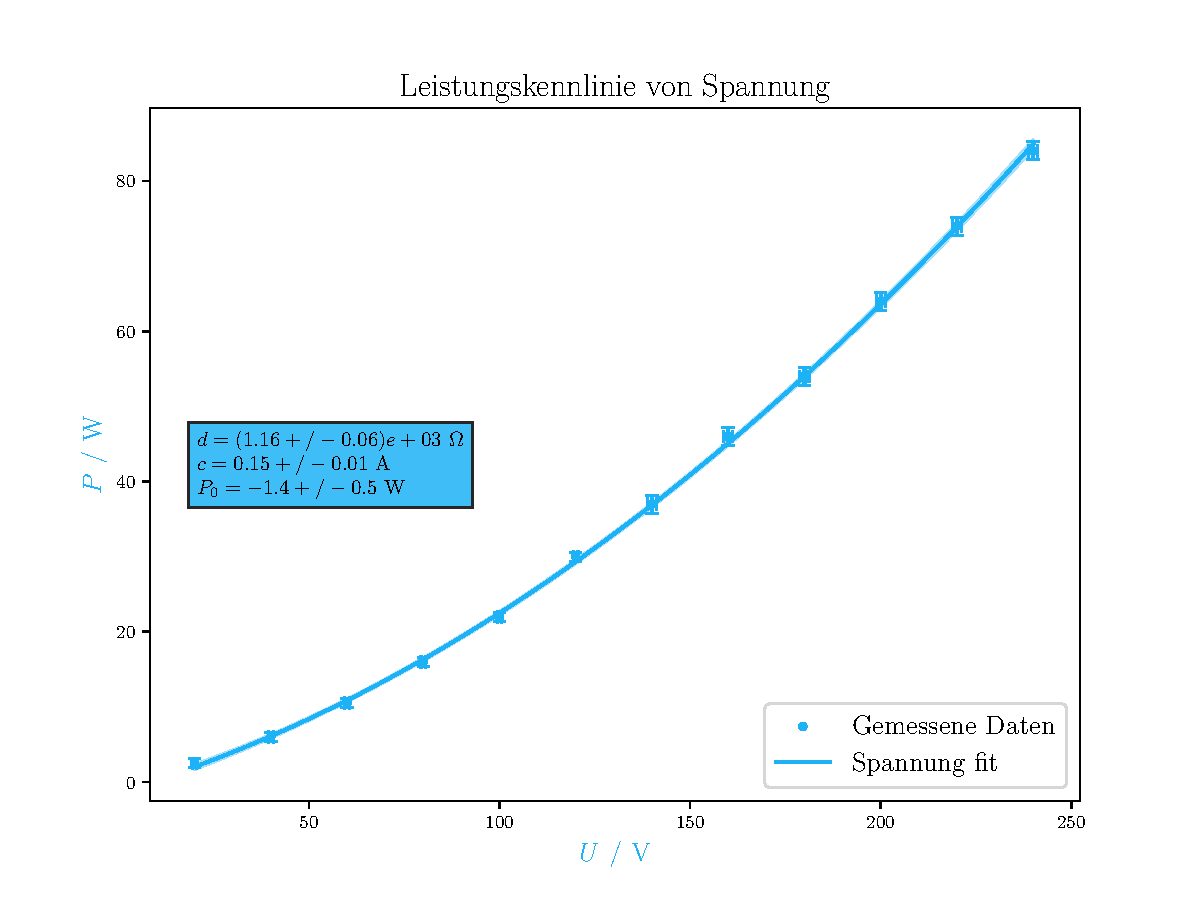
\includegraphics[width = 0.95\textwidth]{figures/pUkennlinie.pdf}
	\end{center}
	\caption[Spannungsabhängige Leistungskurve einer Glühbirne]{ Diese Graphik beinhaltet
		den quadratischen Fit der gemessen Leistungswerte $P$ über die Spannung $U$
		einer Glühbirne, die Werte sind aus \autoref{tab:werte_ohm} entnommen worden.
		Hierbei ist $d$ der gefittete Widerstandswert der Glühbirne, $c$ ist lineare
		Fitparameter und $P_0$ ist der Ordinatenschnitt.
	}\label{fig:pUkennlinie}
\end{figure}

\begin{figure}[H]
	\begin{center}
		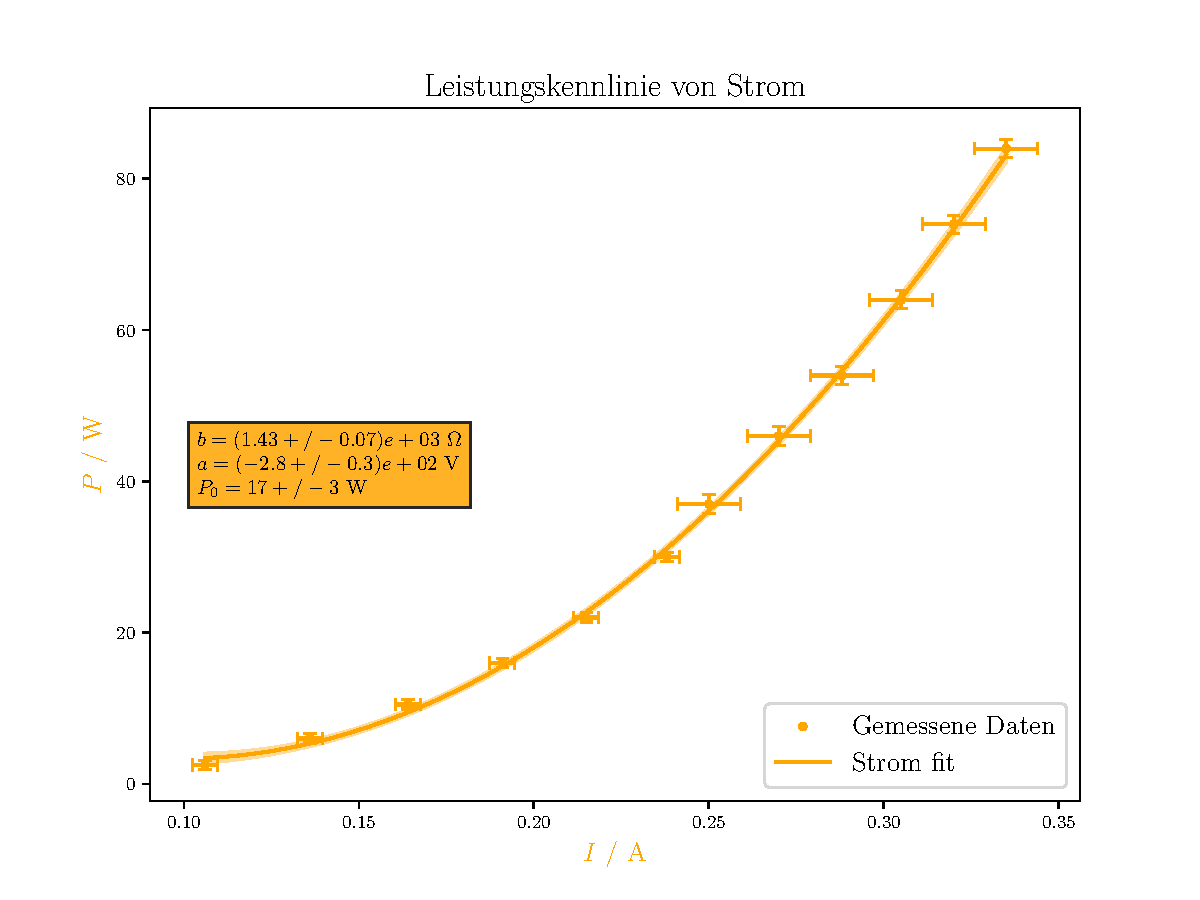
\includegraphics[width = 0.95\textwidth]{figures/pIkennlinie.pdf}
	\end{center}
	\caption[Stromabhängige Leistungskurve einer Glühbirne]{Diese Graphik beinhaltet den
		quadratischen Fit der gemessen Leistungswerte $P$ über die Spannung $U$ einer
		Glühbirne, die Werte sind aus \autoref{tab:werte_ohm} entnommen worden. Hierbei
		ist $d$ der gefittete Widerstandswert der Glühbirne, $c$ ist lineare
		Fitparameter und $P_0$ ist der Ordinatenschnitt.
	}\label{fig:pIkennlinie}
\end{figure}

\subsection{Symmetrische Last in Dreieckschaltung}\label{sec:ausw_dreieck}

Aufgrund der symmetrischen Last lassen sich die Beträge aller Strangströme
$I_{ij}$ mit dem Wissen über die Beträge der Leiterströmen $I_i$ und einem der
Strangströme hier $I_{31}$ bestimmen. Dies lässt sich durch die Komplexe
Vektoraddition der Strangströme berechnen. Dies folgende Umformungen können
gemacht werden da die Winkelverschiebung der Ohmschen Strangströme zu den
Leiterströmen bekannt sind.

\begin{align}
	i_{i}           & = \sum_{j} i_{ij} (1-\delta_{ij})                                                    \\
	I_{i}           & = |\sum_{j} i_{ij} (1-\delta_{ij})|                                                  \\
	\implies I_{12} & = \sqrt{I_1^2-\frac{3I_{31}^2}{4}}-\frac{I_{31}^2}{2}                                \\
	\implies I_{23} & = \sqrt{I_3^2-\frac{3I_{31}^2}{4}}-\frac{I_{31}^2}{2}\label{eq:complexstromaddition}
\end{align}

Mittel dieser Gleichungen lassen sich nun die Beträge der Strangströme
bestimmen.
\begin{table}[H]
	\caption[Errechnete Strangströme bei der Dreiecksschaltung]{ Errechnete Strangströme
		einer symmetrisch ohmsch-belasteten Dreiecksschaltung, siehe
		\autoref{fig:aufbau1}. Zur Berechnung wurde \autoref{eq:complexstromaddition}
		und die Daten aus \autoref{tab:werte_sym_dreieck} entnommen. \\
		$I_{ij} \dots$ errechnete Strangströme vom i-ten zum j-ten Leiter in \si{\ampere}.
	}\label{tab:strangStromDreieck}
	\centering
	\begin{tblr}{colspec={S[table-format=1.2(1)]S[table-format=1.2(1)]S[table-format=1.3(1)]}}
{{{$I_{12}$}}} & {{{$I_{23}$}}} & {{{$I_{31}$}}}\\
{{{\si{\ampere}}}} & {{{\si{\ampere}}}} & {{{\si{\ampere}}}}\\
0.27(3) & 0.28(3) & 0.264(8)\\
\end{tblr}

\end{table}

Mittels der Strangströme (\autoref{tab:strangStromDreieck}) und der
Strangspannungen $U_{ij}$ (\autoref{tab:werte_sym_dreieck}) und der
\autoref{eq:leistung} lassen sich die Verbraucherleistungen der Stränge $P_i$
finden.

\begin{table}[H]
	\caption[Errechnete Leistungen bei der Dreiecksschaltung]{ Errechnete Leistungen bei der
		Dreiecksschaltung                                      \\
		$P_i^C \dots$ errechnete Leistung am i-ten Strang in W \\
		$P_{ges}^C \dots$ errechnete Gesamtleistung in W       \\
		$P_{ges}^M \dots$ gemessene Gesamtleistung in W
	}\label{tab:powerDreieck}
	\centering
	\begin{tblr}{colspec={S[table-format=3.0(2)]S[table-format=3.0(2)]S[table-format=3.0(1)]S[table-format=1.1(1)e3]S[table-format=3.0(1)]}}
{{{$P_1^{C}$}}} & {{{$P_2^{C}$}}} & {{{$P_3^{C}$}}} & {{{$P_{ges}^{C}$}}} & {{{$P_{ges}^{M}$}}}\\
{{{\si{\watt}}}} & {{{\si{\watt}}}} & {{{\si{\watt}}}} & {{{\si{\watt}}}} & {{{\si{\watt}}}}\\
104(12) & 109(12) & 104(6) & 3.2(3)e+02 & 331(7)\\
\end{tblr}

\end{table}

Damit die Rechnungen in \autoref{eq:complexstromaddition} besser
nachzuvollziehen sind wurde von dieser Dreieckschaltung ein Zeigerdiagramm
erstellt.

\begin{figure}[H]
	\begin{center}
		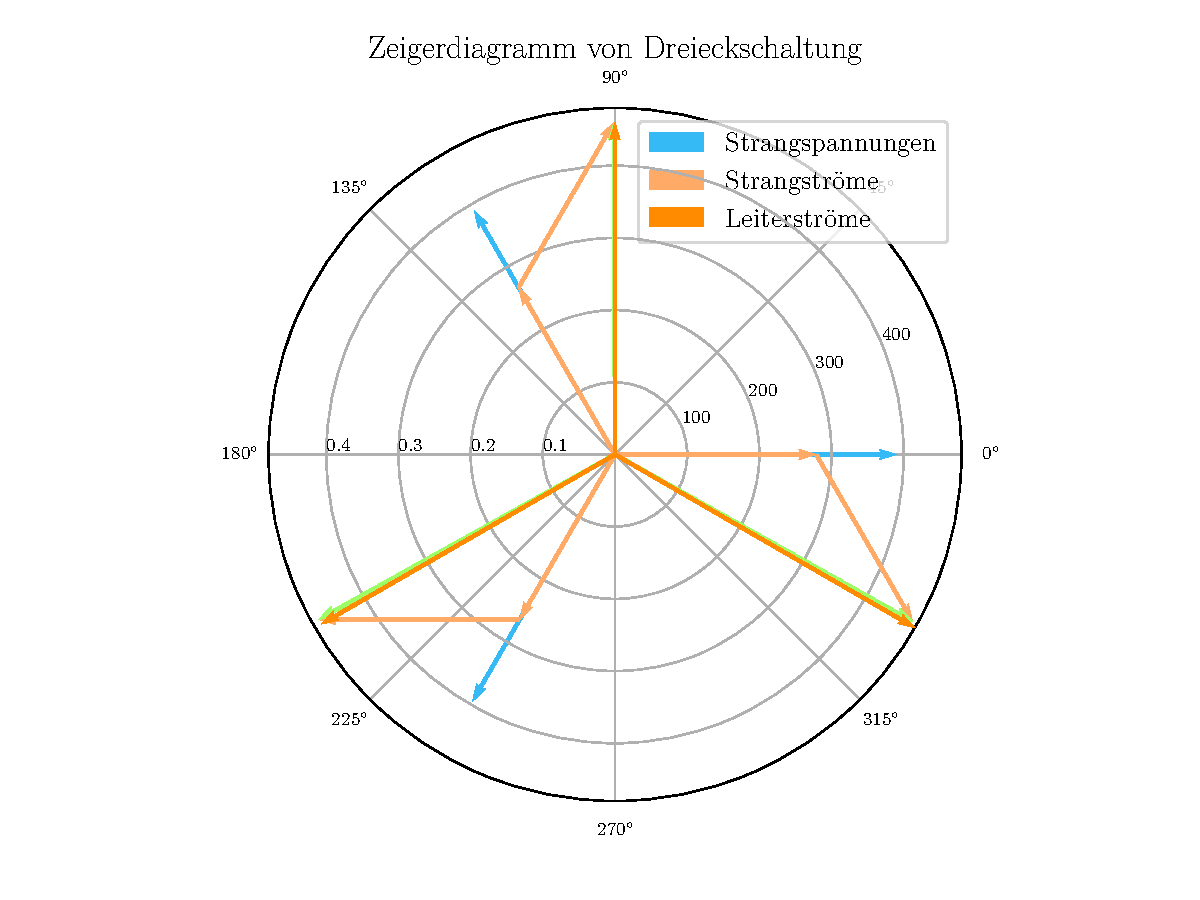
\includegraphics[width = 0.95\textwidth]{figures/zeigerDreieck.pdf}
	\end{center}
	\caption[Zeigerdiagramm einer sysmetrisch ohmsch-belastete Dreieckschaltung]{ Dieses
		Diagramm widerspiegelt die Schaltung, aus \autoref{fig:aufbau1} und wurde mit
		den Werten aus \autoref{tab:strangStromDreieck}, \autoref{tab:werte_ohm}
		erstellt.
	}\label{fig:zeigerDreieck}
\end{figure}

\subsection{Sternschaltungen}\label{sec:aus_stern}

Analog wie in \autoref{sec:ausw_dreieck} werden mittels auch die Strangströme
$I_j$ und Strangspannungen $U_j$ die Verbraucherleistungen der nächsten drei
Sternschaltungen berechnet. Desweitern wird auch mittels der gemessen
Leistungswerte $P_i^M$, \autoref{tab:wert_stern}, die gesamte
Verbraucherleistung bestimmt $P_{ges}^{M}$.

\begin{table}[H]
	\caption[Errechnete Leistungen bei der Sternschaltung]{Errechnete Leistungen bei der
		Sternschaltung                                                    \\
		1. Zeile \dots symmetrische Belastung                             \\
		2. Zeile \dots asymmetrische Belastung                            \\
		3. Zeile \dots asymmetrische Belastung mit simulierten Kabelbruch \\
		$P_i^C \dots$ errechnete Leistung am i-ten Strang in W            \\
		$P_{ges}^C \dots$ errechnete Gesamtleistung in W                  \\
		$P_{ges}^M \dots$ gemessene Gesamtleistung in W
	}\label{tab:powerStern}
	\centering
	\begin{tblr}{colspec={S[table-format=2.0(1)]S[table-format=2.0(1)]S[table-format=2.0(1)]S[table-format=3.0(2)]S[table-format=3.0(1)]}}
{{{$P_1^{C}$ / \si{\watt}}}} & {{{$P_2^{C}$ / \si{\watt}}}} & {{{$P_3^{C}$ / \si{\watt}}}} & {{{$P_{ges}^{C}$ / \si{\watt}}}} & {{{$P_{ges}^{M}$ / \si{\watt}}}}\\
50(2) & 50(2) & 51(3) & 150(7) & 143(3)\\
62(5) & 59(5) & 39(3) & 159(11) & 156(4)\\
52(4) & 57(4) & 48(3) & 156(11) & 162(4)\\
\end{tblr}

\end{table}

Nun wird auch die symmetrisch ohmsch-belastete Sternschaltungen als
Zeigerdiagramm dargestellt. Die hierfür verwendeten Werte sind der
\autoref{tab:wert_stern} entnommen worden, zudem wurde die Phasenverschiebung
zwischen den Leitern als \SI{120}{\degree} vom Stromnetz angenommen.

\begin{figure}[H]
	\begin{center}
		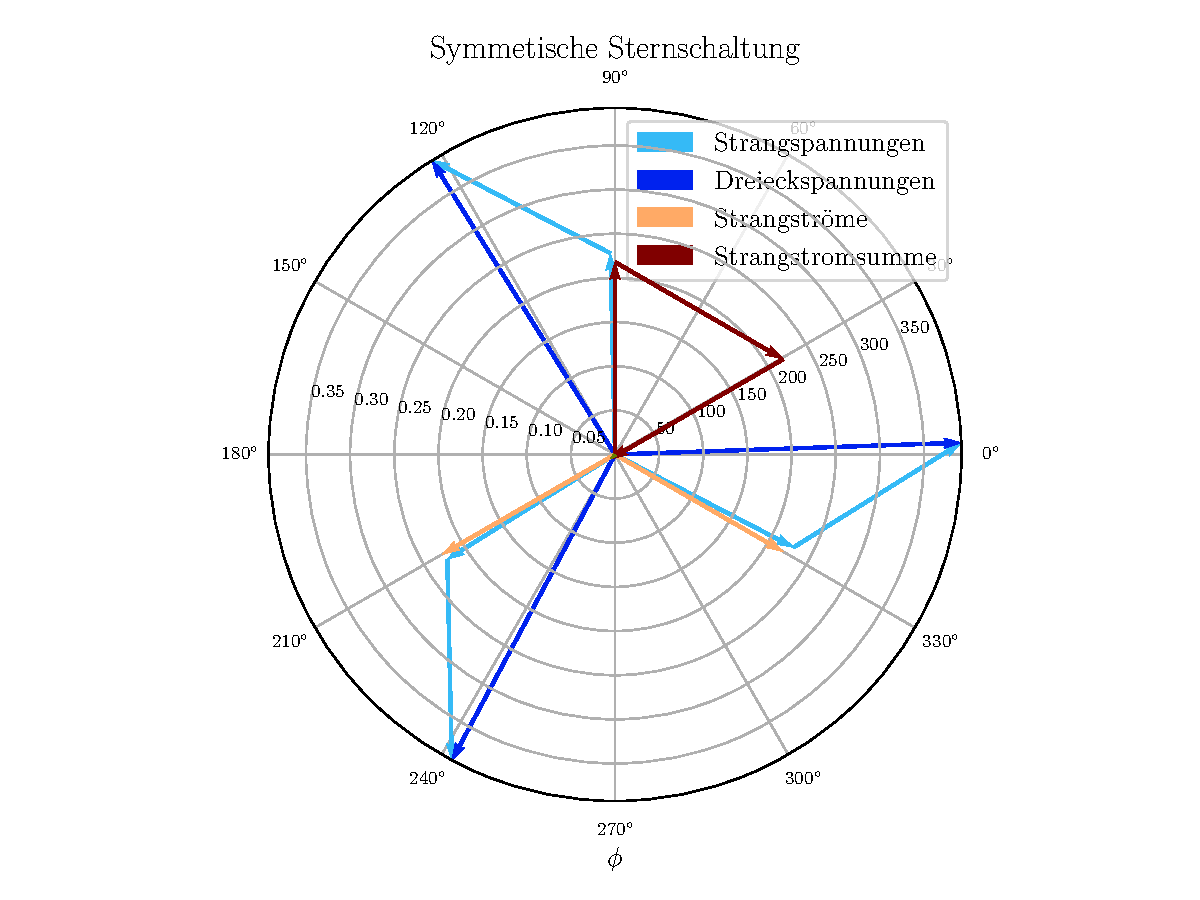
\includegraphics[width = 0.95\textwidth]{figures/zeigerSternSym.pdf}
	\end{center}
	\caption[Zeigerdiagramm einer symmetrisch ohmsch-belastete Sternschaltung]{Dieses
		Diagramm widerspiegelt die Schaltung, aus \autoref{fig:aufbau2} j und wurde mit
		den Werten aus \autoref{tab:wert_stern} erstellt.
	}\label{fig:zeigerSternSym}
	%  Hier ist kein Neutralleiterstrom durch Stromaddition ersichtlich
\end{figure}

Nun galt es mittels des Zeigerdiagramms der asymmetrischen ohmsch-belasteten
Sternschaltungen ohne Neutralleiterbruch den Neutralleiterstrom $I_0$ zu
bestimmen. Dies wurde durch Addition der Strangströme bewerkstelligt.

\begin{figure}[H]
	\begin{center}
		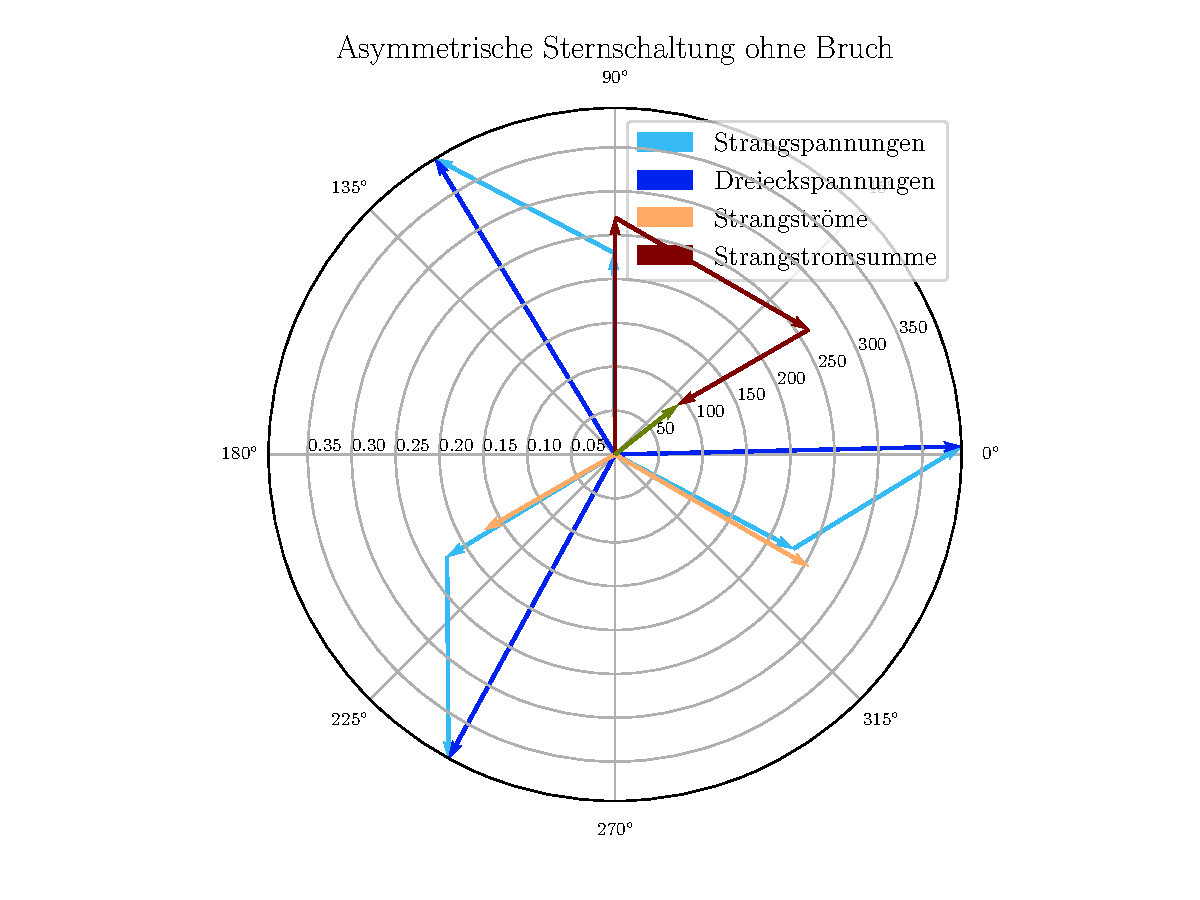
\includegraphics[width = 0.95\textwidth]{figures/zeigerSternAsymOhneBruch.pdf}
	\end{center}
	\caption[Zeigerdiagramm einer asymmetrisch ohmsch-belastete Sternschaltung ohne
		Neutralleiterbruch]{Dieses Diagramm widerspiegelt die asymmetrische
		Sternschaltung mit einem Aufbau, wie in \autoref{fig:aufbau2} ersichtlich.
		Diese wurde, wie in \autoref{sec:vers_asy_stern_ohne} erklärt, modifiziert.
		Hier ist durch die Vektoraddition der Strangströme der Neutralleiterstrom $I_0$
		grünlich dargestellt worden. Die Werte stammen aus \autoref{tab:wert_stern}.
	}\label{fig:zeigerSternAsymOhneBruch}
\end{figure}

Dazu ergänzend wurde auch der Leiterbruch des asymmetrischen ohmsch-belasteten
Sternschaltungen als Zeigerdiagramm dargestellt, damit die
Sternpunktsverschiebung visualisiert wird. Damit die Phasenverschiebung der
Strangspannungen $U_i$ bestimmt werden konnte ist der Kosinussatz, beim Dreieck
der Vektoraddition der $u_i$ zu den Dreieckspannungen $u_{ij} = u_i-u_j =
	400\exp(i\frac{2\pi\cdot(j)}{3}\pi)$, angewendet worden. Schlussendlich konnte
durch die Addition der Strangspannungen $u_i$ mit den Spannungen vom Leiter zu
Neutralleiter $u_{jN} =
	\frac{400}{\sqrt{3}}\exp(i\frac{2\pi\cdot(j+\frac{3}{2})}{3}\pi)$ die
Sternpunktsverschiebung $U_0$ mittels der \autoref{fig:zeigerSternAsymBruch}
bestimmt werden. Dies ist für alle Drei möglich Spannungsadditionen durch
geführt worden, deshalb sind drei Neutralleiterspannungen $U_0$ in
\autoref{fig:zeigerSternAsymBruch} ersichtlich.

\begin{figure}[H]
	\begin{center}
		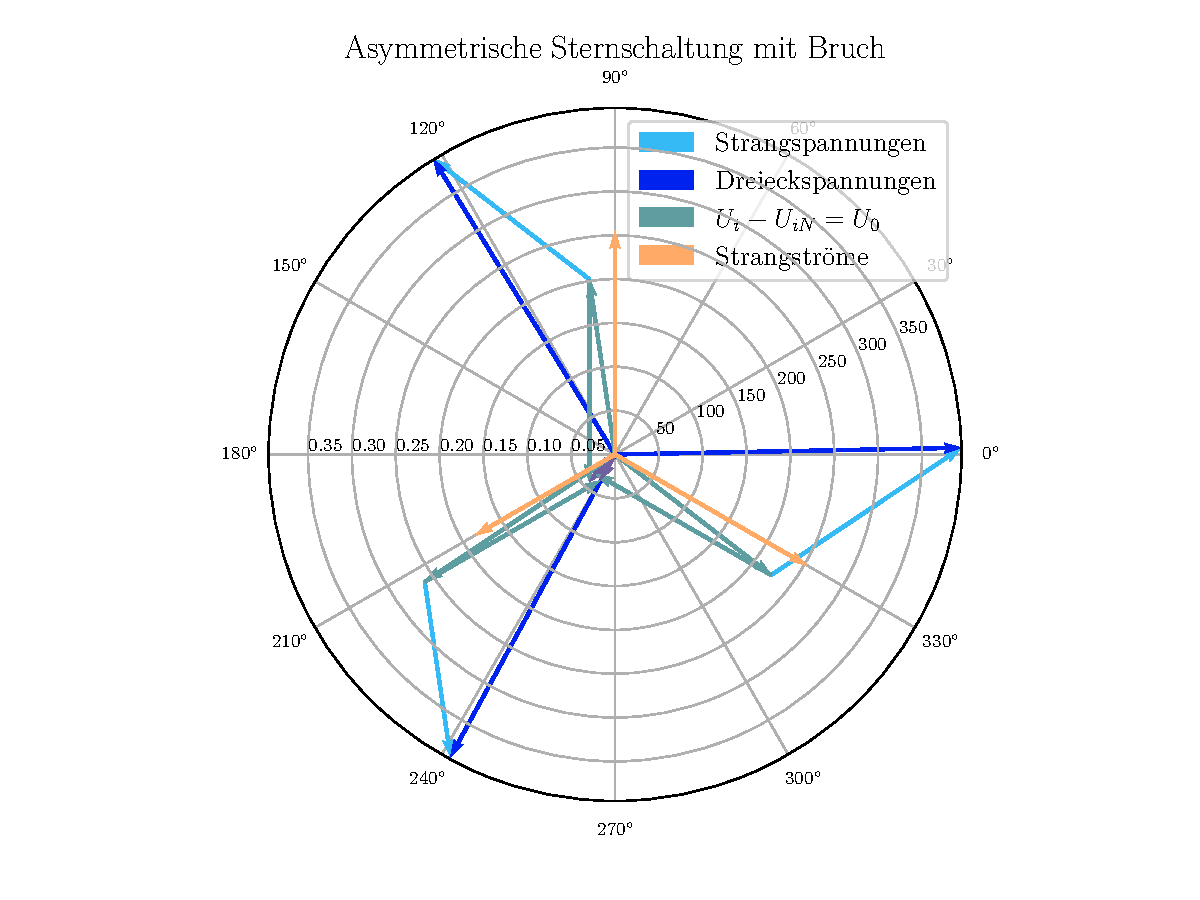
\includegraphics[width = 0.95\textwidth]{figures/zeigerSternAsymBruch.pdf}
	\end{center}
	\caption[Zeigerdiagramm einer asymmetrisch ohmsch-belastete Sternschaltung mit
		Neutralleiterbruch]{Dieses Diagramm widerspiegelt eine asymmetrische
		Sternschaltung mit Neutralleiterbruch mit einem Aufbau, wie in
		\autoref{fig:aufbau2} ersichtlich. Diese wurde, wie in
		\autoref{sec:vers_asy_stern_mit} erklärt, modifiziert. Hier ist durch die
		Vektoraddition der Strangspannungen $U_i$ und der Spannungen vom Leiter zum
		Neutralleiter $U_{iN}$ die Neutralleiterspannungen $U_0$ in der Farbe Lavendel
		dargestellt worden. Die Werte stammen aus \autoref{tab:wert_stern}.
	}\label{fig:zeigerSternAsymBruch}
\end{figure}

\subsection{Wirk- und Blindleistungsmessung bei allgemeiner Last im Dreiphasennetz}

Analog wie in \autoref{sec:aus_stern} sind die Verbraucherleistung $P_i^C$,
durch Multiplikation der Strangströme $I_i$ und der Strangspannungen bestimmt
worden. Zudem wurden auch die Verbraucherblindleistungen $Q_i^C$ bestimmt indem
auch die $I_i$ und die $U_i$ mit einander multipliziert worden sind. Jedoch ist
der Unterschied in der Berechnung, dass bei den $P_i^C$ nur die Reellen Anteile
der Strangspannungen $U_i$ zur Berechnung genommen werden heist Spannungen über
die Widerstände und bei den $Q_i^C$ nur die Imaginären Anteile der
Strangspannungen $U_i$ (Kondensator- \& Indukturspannungen der Stränge) zur
Berechnung genommen werden. Des Weiteren wurden auch die gesamt
Verbraucherleistung $P_{ges}$ und die gesamt Verbraucherblindleistung $Q_{ges}$
bestimmt. Einmal durch die Summation der gemessenen Verbraucherleistung $P_i^M$
und der gemessenen Verbraucherblindleistung $Q_i^M$ (aus
\autoref{tab:werte_wirkleistung}) und einmal durch die Summation der
errechneten Werte ($P_i^C$ \& $Q_i^C$).

\begin{table}[H]
	\caption[Errechnete Werte für die Wirk- und Blindleistungen bei allgemeiner Last]
	{\footnotesize Errechnete Werte für die Wirk- und Blindleistungen, sowie
		gegenüberstellung mit dem gemessenen Wert bei allgemeiner Last, jeweils pro
		Block:                                                                                        \\
		1. Zeile \dots entsprechende Parameter bei Versuchsaufbau nach
		\autoref{fig:aufbau3}                                                                         \\
		2. Zeile \dots entsprechende Parameter bei Versuchsaufbau mit vertauschten
		Außenleitern                                                                                  \\
		3. Zeile \dots entsprechende Parameter bei Versuchsaufbau bei modifizierter
		Schaltung                                                                                     \\
		$P_i^C \dots$ Errechnete Wirkleistung am i-ten Strang in W (im 1. Block aus den
		gemessenen Werten der Wirkleistung, im 4. Block aus den gemessenen Werten der Scheinleistung) \\
		$P_i^M \dots$ Gemessene Wirkleistung am i-ten Strang in W                                     \\
		$P_{ges}^C \dots$ Errechnete gesamte Wirkleistung in W                                        \\
		$P_{ges}^M \dots$ Gemessene gesamte Wirkleistung in W                                         \\
		$Q_i^C \dots$ Errechnete Scheinleistung am i-ten Strang in W (im 2. Block aus den
		gemessenen Werten der Scheinleistung, im 3. Block aus den gemessenen Werten der Wirkleistung) \\
		$Q_i^M \dots$ Gemessene Scheinleistung am i-ten Strang in W                                   \\
		$Q_{ges}^C \dots$ Errechnete gesamte Scheinleistung in W                                      \\
		$Q_{ges}^M \dots$ Gemessene gesamte Scheinleistung in W
	}\label{tab:powerAufgabe3}
	\begin{tblr-x}{cells={font=\footnotesize},row{1}={font=\mathversion{bold}\footnotesize},colspec={S[table-format=3.0(2)]S[table-format=3.0(1)]S[table-format=3.0(2)]S[table-format=3.1(3)]S[table-format=1.1(1)e1]S[table-format=3.1(3)]}}
{{{$P_1^{C}$ / \si{\watt}}}} & {{{$P_1^{M}$ / \si{\watt}}}} & {{{$P_2^{C}$ / \si{\watt}}}} & {{{$P_2^{M}$ / \si{\watt}}}} & {{{$P_3^{C}$ / \si{\watt}}}} & {{{$P_3^{M}$ / \si{\watt}}}}\\
353(18) & 370(4) & 69(5) & 69.0(16) & 3.2(3)e+02 & 345(7)\\
359(18) & 375(4) & 70(5) & 70.0(16) & 3.2(3)e+02 & 340(7)\\
359(18) & 375(4) & 332(18) & 345(7) & 1.6(1)e+02 & 86.0(16)\\
\end{tblr-x}

	\vskip -25.3pt
	\begin{tblr-x}{cells={font=\footnotesize},row{1}={font=\mathversion{bold}\footnotesize},colspec={S[table-format=1.1(1)]S[table-format=1.3(1)]S[table-format=2.1(3)]S[table-format=2.1(3)]S[table-format=2.0(1)]S[table-format=3.1(3)]}}
{{{$Q_1^{C}$ / \si{\Var}}}} & {{{$Q_1^{M}$ / \si{\Var}}}} & {{{$Q_2^{C}$ / \si{\Var}}}} & {{{$Q_2^{M}$ / \si{\Var}}}} & {{{$Q_3^{C}$ / \si{\Var}}}} & {{{$Q_3^{M}$ / \si{\Var}}}}\\
0.0(0) & 0.289(3) & 28.5(18) & 28(1) & 69(4) & 67(1)\\
0.0(0) & 0.289(3) & 28.3(18) & 28(1) & 69(4) & 71.6(19)\\
0.0(0) & 0.577(6) & 81(6) & 80.8(19) & 84(4) & 156(4)\\
\end{tblr-x}

	\vskip -25.3pt
	\begin{tblr-x}{cells={font=\footnotesize},row{1}={font=\mathversion{bold}\footnotesize}{cyan7},colspec={S[table-format=1.1(1)]S[table-format=2.1(3)]S[table-format=3.0(1)]S[table-format=2.0(1)e1]S[table-format=1.1(1)e1]S[table-format=3.0(2)]}}
{{{$Q_1^{C}$ / \si{\Var}}}} & {{{$Q_2^{C}$ / \si{\Var}}}} & {{{$Q_3^{C}$ / \si{\Var}}}} & {{{$Q_{ges}^{C}$ / \si{\Var}}}} & {{{$P_{ges}^{C}$ / \si{\watt}}}} & {{{$P_{ges}^{M}$ / \si{\watt}}}}\\
0.0(0) & -27.5(17) & 114(6) & 87(8) & 7.4(5)e+02 & 784(12)\\
0.0(0) & -27.9(18) & 69(4) & 41(6) & 7.5(5)e+02 & 785(12)\\
0.0(0) & -81(6) & 85(4) & 0(1)e+01 & 8.5(5)e+02 & 806(12)\\
\end{tblr-x}

	\vskip -25.3pt
	\begin{tblr-x}{cells={font=\footnotesize},row{1}={font=\mathversion{bold}\footnotesize},colspec={S[table-format=3.0(2)]S[table-format=3.0(2)]S[table-format=1.1(1)e1]S[table-format=1.1(1)e1]S[table-format=2.1(1)e1]S[table-format=3.1(3)]}}
{{{$P_1^{C}$ / \si{\watt}}}} & {{{$P_2^{C}$ / \si{\watt}}}} & {{{$P_3^{C}$ / \si{\watt}}}} & {{{$P_{ges}^{C}$ / \si{\watt}}}} & {{{$Q_{ges}^{C}$ / \si{\Var}}}} & {{{$Q_{ges}^{M}$ / \si{\Var}}}}\\
359(18) & 72(5) & 3.2(3)e+02 & 7.5(5)e+02 & 98(6) & 95.0(19)\\
359(18) & 71(5) & 3.2(3)e+02 & 7.5(5)e+02 & 97(6) & 100(3)\\
359(18) & 330(18) & 1.6(1)e+02 & 8.4(5)e+02 & 1.6(1)e+02 & 237(6)\\
\end{tblr-x}

\end{table}

Schlussendlich kann mit den $P_{ges}$ und den gesamt $Q_{ges}$ die gesamte
Scheinleistung mit Pythagoras berechnet werden.

\begin{table}[H]
	\caption[Errechnete Werte für die Scheinleistungen bei allgemeiner Last] { Errechnete
		Werte für die Scheinleistungen, sowie gegenüberstellung mit dem gemessenen Wert
		bei allgemeiner Last, jeweils pro Block:                        \\
		1. Zeile $\dots$ entsprechende Parameter bei Versuchsaufbau nach
		\autoref{fig:aufbau3}                                           \\
		2. Zeile $\dots$ entsprechende Parameter bei Versuchsaufbau mit vertauschten
		Außenleitern                                                    \\
		3. Zeile $\dots$ entsprechende Parameter bei Versuchsaufbau bei modifizierter
		Schaltung                                                       \\
		$S_{ges}^C \dots$ Errechnete gesamte Scheinleistung in \si{\VA} \\
		$S_{ges}^M \dots$ Gemessene gesamte Scheinleistung in \si{\VA}  \\
	}\label{tab:scheinleistung}
	\centering
	\begin{tblr}{cells={font=\footnotesize},row{1}={font=\mathversion{bold}\footnotesize},colspec={S[table-format=1.1(1)e1]S[table-format=3.0(2)]}}
{{{$S_{ges}^{C}$ / \si{\VA}}}} & {{{$S_{ges}^{M}$ / \si{\VA}}}}\\
7.5(5)e+02 & 785(12)\\
7.5(5)e+02 & 786(12)\\
8.4(5)e+02 & 810(13)\\
\end{tblr}

\end{table}

Nun wird werden die Messungen von der Standardschaltung, siehe
\autoref{fig:aufbau3}, und der Messungen mit den Außenleitern L2 und L3
vertauscht in einem Zeigerdiagramm dargestellt. Um die Phasenverschiebung der
Spannungen zu finden wurde der Satz von Pythagoras verwendet, dies ist auch in
\autoref{fig:zeigerSternReal} ersichtlich.

\begin{figure}[H]
	\begin{center}
		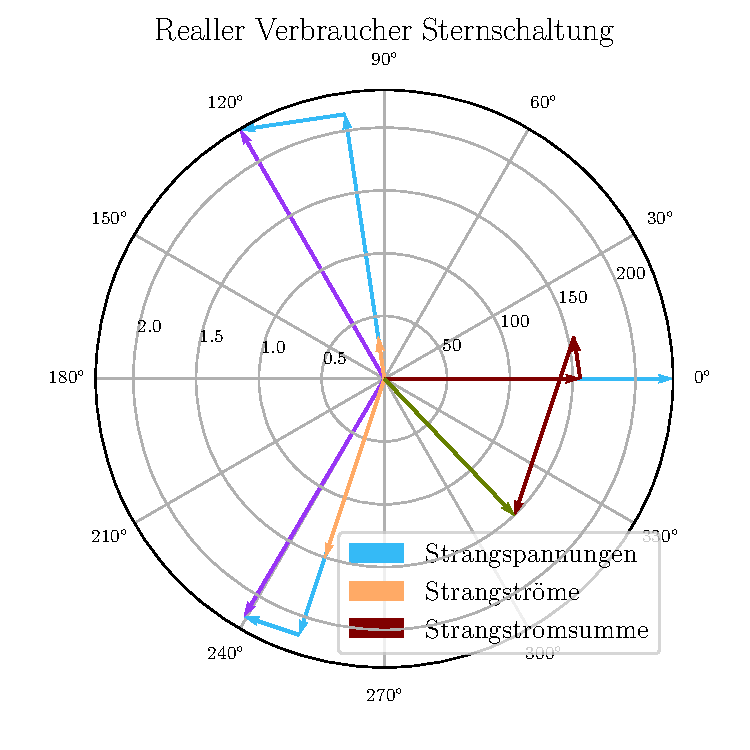
\includegraphics[width = 0.48\textwidth]{figures/zeigerSternReal.pdf}
		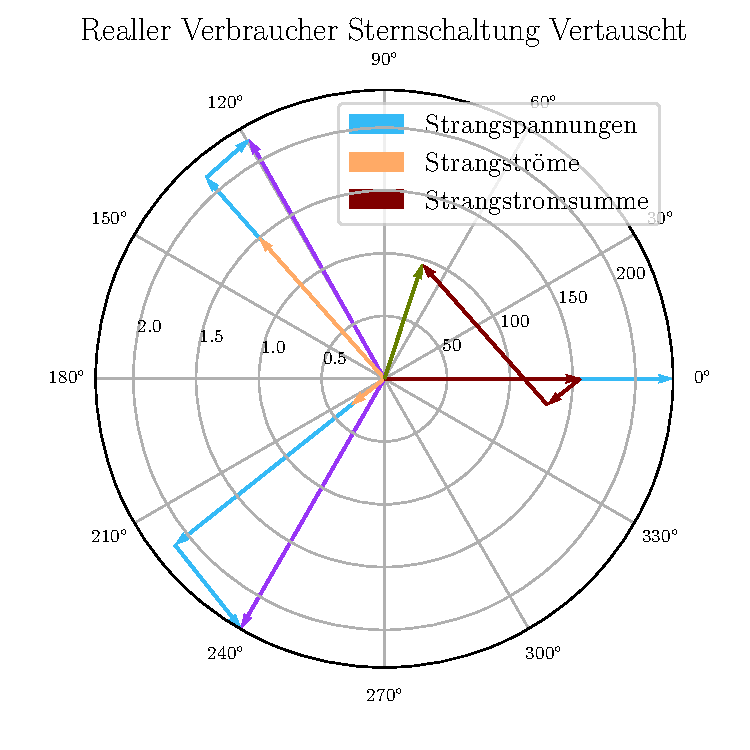
\includegraphics[width = 0.48\textwidth]{figures/zeigerSternRealVertauscht.pdf}
	\end{center}
	\caption[Zeigerdiagramme einer real-belastete Sternschaltung und dessen vertauschten
		Leiter]{Diese Diagramme widerspiegeln die real-belastete Sternschaltung mit
		einem Aufbau, wie in \autoref{fig:aufbau3} ersichtlich. Wobei beim Vertauschten
		die Leiter 2 und 3 vertauscht wurden. Hier ist durch die Vektoraddition der
		Strangströme der Neutralleiterstrom $I_0$ grünlich dargestellt worden. Die
		Werte stammen aus \autoref{tab:werte_wirkleistung}.
	}\label{fig:zeigerSternReal}
\end{figure}

%1. Zeile \dots Wirkleistung eines realen Verbrauchers, errechnet aus den gemessenen Wirkleistungen\\
%	2. Zeile \dots Wirkleistung eines realen Verbrauchers mit vertauschten
%	Außenleitern, errechnet aus den gemessenen Wirkleistungen          \\
%	3. Zeile \dots Wirkleistung bei modifizierter Schaltung, errechnet aus den gemessenen Wirkleistungen\\
%	4. Zeile \dots Blindleistung eines realen Verbrauchers, errechnet aus den gemessenen Scheinleistungen\\
%	5. Zeile \dots Blindleistung eines realen Verbrauchers mit vertauschten
%	Außenleitern, errechnet aus den gemessenen Scheinleistungen                                  \\
%	6. Zeile \dots Blindleistung bei modifizierter Schaltung, errechnet aus den gemessenen Scheinleistungen\\
%	7. Zeile \dots Blindleistung eines realen Verbrauchers, errechnet aus den gemessenen Wirkleistungen\\
%	8. Zeile \dots Blindleistung eines realen Verbrauchers mit vertauschten
%	Außenleitern, errechnet as den gemessenen Wirkleistungen          \\
%	9. Zeile \dots Blindleistung bei modifizierter Schaltung , errechnet aus den gemessenen Wirkleistungen\\
%	10. Zeile \dots Wirkleistung eines realen Verbrauchers, errechnet aus den gemessenen Scheinleistungen\\
%	11. Zeile \dots Wirkleistung eines realen Verbrauchers mit vertauschten
%	Außenleitern, errechnet aus den gemessenen Scheinleistungen                             \\
%	12. Zeile \dots Wirkleistung bei modifizierter Schaltung, errechnet aus den gemessenen Scheinleistungen\\

\subsection{Bau eines rudimentären Asynchron-Drehstrommotors}

Hier ist keine Auswertung von Nöten.

\section{Diskussion}\label{sec:diskussion}

\subsection{ohmsche Last in Wechselstromkreis}

Wie in \autoref{fig:pIkennlinie} und \autoref{fig:pUkennlinie} ersichtlich
lässt sich das Verhalten der Leistung gut durch beide quadratischen Funktionen
$P(I)$ (\autoref{eq:fitstrom}) und $P(U)$ (\autoref{eq:fitspannung})
beschreiben. Jedoch wenn die Fitparameter der Fits sich anschaut ist klar
ersichtlich, dass $P(U)$ das Verhalten physikalisch Akkurater, da der Bais
$P_0$ hier kleiner ist. Zudem ist ein leichter Trend in den Bildern zu
erkennen, dass bei höherer Temperatur der Widerstandswert steigt. Da die Lampe
vorgewärmt wurde ist dies jedoch kaum ersichtlich. Durch Höhere Leistung wird
mit einer Verzögerung auch der Metalldraht in der Glühbirne erhitzt, welcher
sich wie ein PTC verhaltet und höherer Temperatur an Widerstand zunimmt.

\subsection{Symmetrische Last in Dreieckschaltung vs in Sternschaltung}
% • Bauen Sie weiterhin unter symmetrischer Last eine Sternschaltung nach Abb. 2 auf und
% messen abermals die Verbraucherleistungen.
% • Welche Unterschiede sind f¨ur die beiden Verkettungen zu beobachten?

Wie zu erwarten ist der Leistungwert der Dreieckschaltung höher als bei der
Sternschaltung. Das Verhältnis der Leistungen sollte bei einem idealen ohmschen
symmetrischen Belastung zwischen Dreieckschaltung und Sternschaltung 3
betragen.

\begin{equation}
	\frac{P_{ges\triangle}^M}{P_{ges\star}^M} = \num{2.31(7)}
\end{equation}

Wie man sieht ist dieser Wert kleiner als 3, was mit dem gemessenen und
gefitteten Leistungsverhalten einer Glühbirne erklären ist. Die Glühbirnen
verhalten sich nicht wie ein idealer ohmsche Last sondern werden weniger
Leitfähig zunehmender Leistung zu.

\subsection{Sternschaltung sym. vs asym. vs asym. mit Bruch}
% • Welchen Unterschied k¨onnen Sie beim Vergleich der beiden Gesamtleistungen jeder Mes-
% sung erkennen und worin begr¨undet sich dieser?
% – Zeichnen Sie hierf¨ur auch zwei Zeigerdiagrame: einmal aller Str¨ome (mit I0) f¨ur
% den unsymmetrischen Fall mit Strommessger¨at im Neutralleiter und einmal mit den
% aufgenommenen Spannungen (mit U0) f¨ur den unsymmetrischen Fall mit Spannungs-
% messger¨at im Neutralleiter .
% – Vergleichen Sie die beiden gemessenen Werte mit den beiden sich aus der Zeichnung

\subsection{Allgemeine Last in Sternschaltung}
% • Vertauschen Sie die Außenleiter L2 und L3 und notieren Sie die eventuell auftretende
% Ver¨anderung (Was ist der Grund f¨ur diese Ver¨anderung?).
% • Erstellen Sie zu den Messreihen (Standard + mit vertauschten Außenleiter) je ein Zei-
% gerdiagramm f¨ur alle Str¨ome und Spannungen, die in der Schaltung auftreten. Dies kann
% pro Messreihe entweder getrennt in ein Strom- und ein Spannungsdiagramm erfolgen,
% oder beides zusammengefasst in ein Diagramm dargestellt werden.
% • Errechnen Sie aus den gemessenen Leistungen die am gesamten Verbraucher abfallenden
Durch die Vertauschung der Leiter L2 \& L3 ist der Nullleiterstrom $I_0$
gesunkten, alle anderen Größen bleiben dabei unverändert. Da die
Phasenverschiebung zwischen den Leitern bei den Blindwiderständen vom
Kondensator und Spule einen Unterschied in der Phasenverschiebung der Ströme
auch verursacht, demzufolge ändert sich auch die Summe der Strangströme, das
beschriebene Verhalten ist in \autoref{fig:zeigerSternReal} zu sehen.

% TODO Messfehler Q_3 Matthias

\subsection{Bau eines rudimentären Asynchron-Drehstrommotors}
% • Realisieren Sie mittels drei Spulen samt Eisenkern mit vorgeschalteten Heizwiderst¨anden
% und einer horizontal gelagerten metallenen Drehscheibe eine rudiment¨are Asynchron-
% Drehstrommaschine in Sternschaltung.
% • Diskutieren Sie die prinzipielle Funktionsweise eines Asynchron- Drehstrommotors und

Nach Absprache mit dem Betreuer war der bisherige Rekord für die maximale
Drehzahl bisher 680 Umdrehungen pro Minute, was mit unserem Ergebnis von 1691
beachtlich gesteigert werden konnte. Dies wurde vor allem durch feine
Anpassungen der Eisenkerne und auch eine Schmierung der Metallscheibe durch
Seife erreicht.

\section{Zusammenfassung}\label{sec:zusammenfassung}

\subsection{ohmsche Last in Wechselstromkreis}

\subsection{Symmetrische Last in Dreieckschaltung}

\subsection{Sternschaltungen}

\subsection{Asymmetrische Last in Sternschaltung}

\subsection{Asymmetrische Last in Sternschaltung und simulierten Kabelbruch}

\subsection{Wirkleistungsmessung}

\subsection{Blindleistungsmessung}

\subsection{Bau eines rudimentären Asynchron-Drehstrommotors}

\newpage

% \printbibliography
\listoffigures
\listoftables
\end{document}
